

\appendix

\section{The \EnDD \ Algorithm}
\label{sec:the-endd-algorithm}

The original paper features an excellent description of the mathematical formulation of the \EnDD \ model, but we did not find it immediately obvious how to translate this into an implementation in a modern deep learning framework. For this reason, we will now briefly describe it from an algorithmic-centred perspective using pseudocode and plain English.  

The process of training an \EnDD \ model is described in Algorithm 1. In practice, the optimization in line 7 can easily be achieved using the standard "fit" method of frameworks such as Keras and PyTorch, by constructing an intermediate dataset and using a custom loss function with a callback for annealing the temperature. 

The intermediate dataset is constructed by first adding any auxiliary images to the training images, and then passing the extended image set as input to the ensemble. The ensemble should output an array of logits as described in line 5 of Algorithm 1. The new dataset is then formed by matching each image to its corresponding ensemble logits, using the latter as the target. 

The custom loss function is described in Algorithm 2. This formulation includes temperature annealing. This loss function is the only modification necessary to adapt a general classification model into an \EnDD \ model, providing it is then trained on an intermediate dataset as described in the previous paragraph. Note that this formulation assumes that the model outputs logits. This output can be converted into Dirichlet probabilities by applying the standard softmax operation.  

%EnD$^2$ \cite{malinin2019ensemble} builds upon prior networks, a concept from an earlier paper published by the same authors \cite{NIPS2018_7936}. A prior network is a neural network that is trained to predict the parameters $\alpha$ of a Dirichlet distribution $Dir(\alpha)$. A prior network can thus be seen as a distribution over distributions over class probabilities. The purpose of a prior network is to differentiate between data and knowledge uncertainty. The network is trained to represent the two types of uncertainty by the placement and the sharpness of the Dirichlet. \\

%A key question is how to create labels corresponding to the inputs $\mathbf{X}$ given that the classes of the training data are known. The author, in the original PN paper \cite{NIPS2018_7936}, proposes choosing a vector $\mathbf{\alpha}$ where all the elements $\alpha_i$ are 1 except for the $i$ corresponding to the correct class, for which $\alpha_i$ should be chosen “large”. The label vector thus contains the parameters of a sharp distribution located close to the i’th corner of a simplex. The prior network is importantly also trained on OOD images where all the $\alpha_i$'s of the corresponding label are set to 1 which corresponds to a flat Dirichlet. The prior network is trained using KL-divergence between the true and predicted Dirichlet.\\ \\
%EnD$^2$ is a prior network in that it too parameterizes a Dirichlet distribution, however, as opposed to the method discussed above, EnD$^2$ uses a trained ensemble to generate the labels $\mathbf{\alpha}$. The label $\alpha$ corresponding to input image $\mathbf{X}$ is computed as, $\mathbf{\alpha} = e^{\phi}$ , where $\phi$ is the ensemble output corresponding to the image $\mathbf{X}$. Distilling the network into a PN is done by taking $\mathbf{\alpha}$ to be a set of samples from the “true” Dirichlet distribution and minimizing the negative log-likelihood between the ensemble prediction and the PN prediction \textbf{Alg 2}. Importantly this loss function is equivalent to the KL-divergence between the true and predicted Dirichlet. For EnD$^2$ no OOD data is required as ensembles already can differentiate between aleatoric and epistemic uncertainty, it is however shown that using OOD data during the distillation can boost the performance of the prior network. The task of this paper is thus to distil the information of uncertainty present in an ensemble to a single prior network. EnD$^2$ uses temperature annealing to increase the support between the ensemble predictions $\mathbf{\alpha}$ and the predicted Dirichlet $\mathbf{\hat{\alpha}}$ at the start of training. This is done by dividing the output logits of both networks by a constant $T$ i.e. $\alpha_i = e^{z_i/T}$, flattening both distributions. The entire EnD$^2$ training is explained as a pseudocode \textbf{Alg 1}.\\
\begin{algorithm}
    \SetKwInOut{Input}{Input}
    \SetKwInOut{Output}{Output}
    \Input{Ensemble $En$ outputting logits, training data X (same as the ensemble is trained on), (optional) Out of distribution data $X_{OOD}$ }
    \Output{Trained EnD$^2$ model} \\
    \If{$X_{OOD}$ not None}{
    $X = [X, X_{OOD}]$ // append OOD data to training set
    }
    $\phi = En.predict(X)$ // exp($\phi$) are the labels for EnD$^2$  \\
    // $\phi$ is a tensor of logits corresponding to the true distribution, each row corresponds to a model and each column a class. Each matrix corresponds to one image \\
    $model_{\theta} \leftarrow classifier$ //create a new classifier model with weights $\theta$, with logits as output \\
    EnD$^2 = argmin_{\theta}\{Loss_{EnD^2}(\phi,model_{\theta}(X)) \}$ //train model backpropagation\\
    return EnD$^2$
    \caption{Training algorithm for EnD$^2$ given an ensemble}
    \label{alg:training}
    
\end{algorithm} \\
\begin{algorithm}
    \SetKwInOut{Input}{Input}
    \SetKwInOut{Output}{Output}
    \Input{Ensemble logits: $\phi$, predicted logits: $z$, temperature: $T=T(t)$, annealing}
    \Output{cost: $C$}
    $\epsilon = 10^{-8}$  // Smoothing factor\\
    $\delta = 1-10^{-3}$ // Central smoothing factor\\
    
    $\alpha = e^{z/T(t)}$ // elementwise exponential\\
    M = \#models \\
    N = \#classes \\
    \For{$i\gets1$ \KwTo M}{ 
    $\alpha_0_i = \sum_j \alpha_{i,j}$ // sum over the classes to produce the precision factor
    }
    %$\alpha_0 = sum(exp(\phi))$ 
    $P_{En} = softmax(\phi/T(t))$ // softmax over classes\\
    $P_{En} = \delta(P_{En} - \frac{1}{N}) + \frac{1}{N}$\\
    $TIT = \sum_i^N(log(\Gamma(\alpha_i + \epsilon))) - log(\Gamma(
            \alpha_0 + \epsilon))  $ // target independent term, where $log(\Gamma(x)) = log((x - 1)!)$\\
    $A = \frac{1}{M}\sum^{M}_i(log(P_{En_i} + \epsilon)$ // mean over ensemble\\
    $TDT = -\sum_i^{N}((\alpha_i - 1) A_i)$  // target dependent term, sum over classes \\

    return $(TDT +TIT) T(t)^2$
    
    
    \label{alg:loss}
    \caption{loss for EnD$^2$}
    

\end{algorithm} 
\\


\section{Experiments on Synthetic Data}
\label{sec:experiments-on-synthetic-data}

\subsection{Methodology}

The goal with these experiments is to provide qualitative justification for \hyperlink{claim5}{Claim 5} and illustrate the inner workings of \EnDD. We also provide some new experiments on temperature annealing and the size of the auxiliary dataset, to visualize their effect. 

\subsubsection{Dataset}

To illustrate the model, Malinin et. al. use a synthetic dataset in $\mathbb{R}^2$. Our rendering of this dataset can be seen in Figure \ref{fig:2}. This is advantageous since it enables plotting both knowledge and data uncertainty over the entire data manifold, giving a qualitative understanding of whether the algorithm works or not, in contrast to higher dimensional data (images, etc.) that cannot be plotted. The dataset itself looks like a spiral, divided into three classes shaped as spiralling arms of increasing radius. The spirals are centred and almost symmetric around the origin. Furthermore, they have increased noise and overlap with radius, which leads us to believe that uncertainty should vary as well. In addition to the spiral data an OOD data-set, referred to as the AUX data-set is also used, which takes the form of a ring slightly outside the spiral.

For the experiments, 1000 samples per ID class are used, both for training and test. The number of AUX samples was also 1000. This is the same setting as the original paper. The generation of the data uses the original paper's code, but the hyperparameters were not specified. Our hyperparameters can be found in our code. We manually searched for hyperparameters, so that our plot would look as close to theirs, but the exact correspondence is probably not achieved. 

\begin{figure}
    \centering
    \begin{subfigure}{0.4\textwidth}
      \centering
      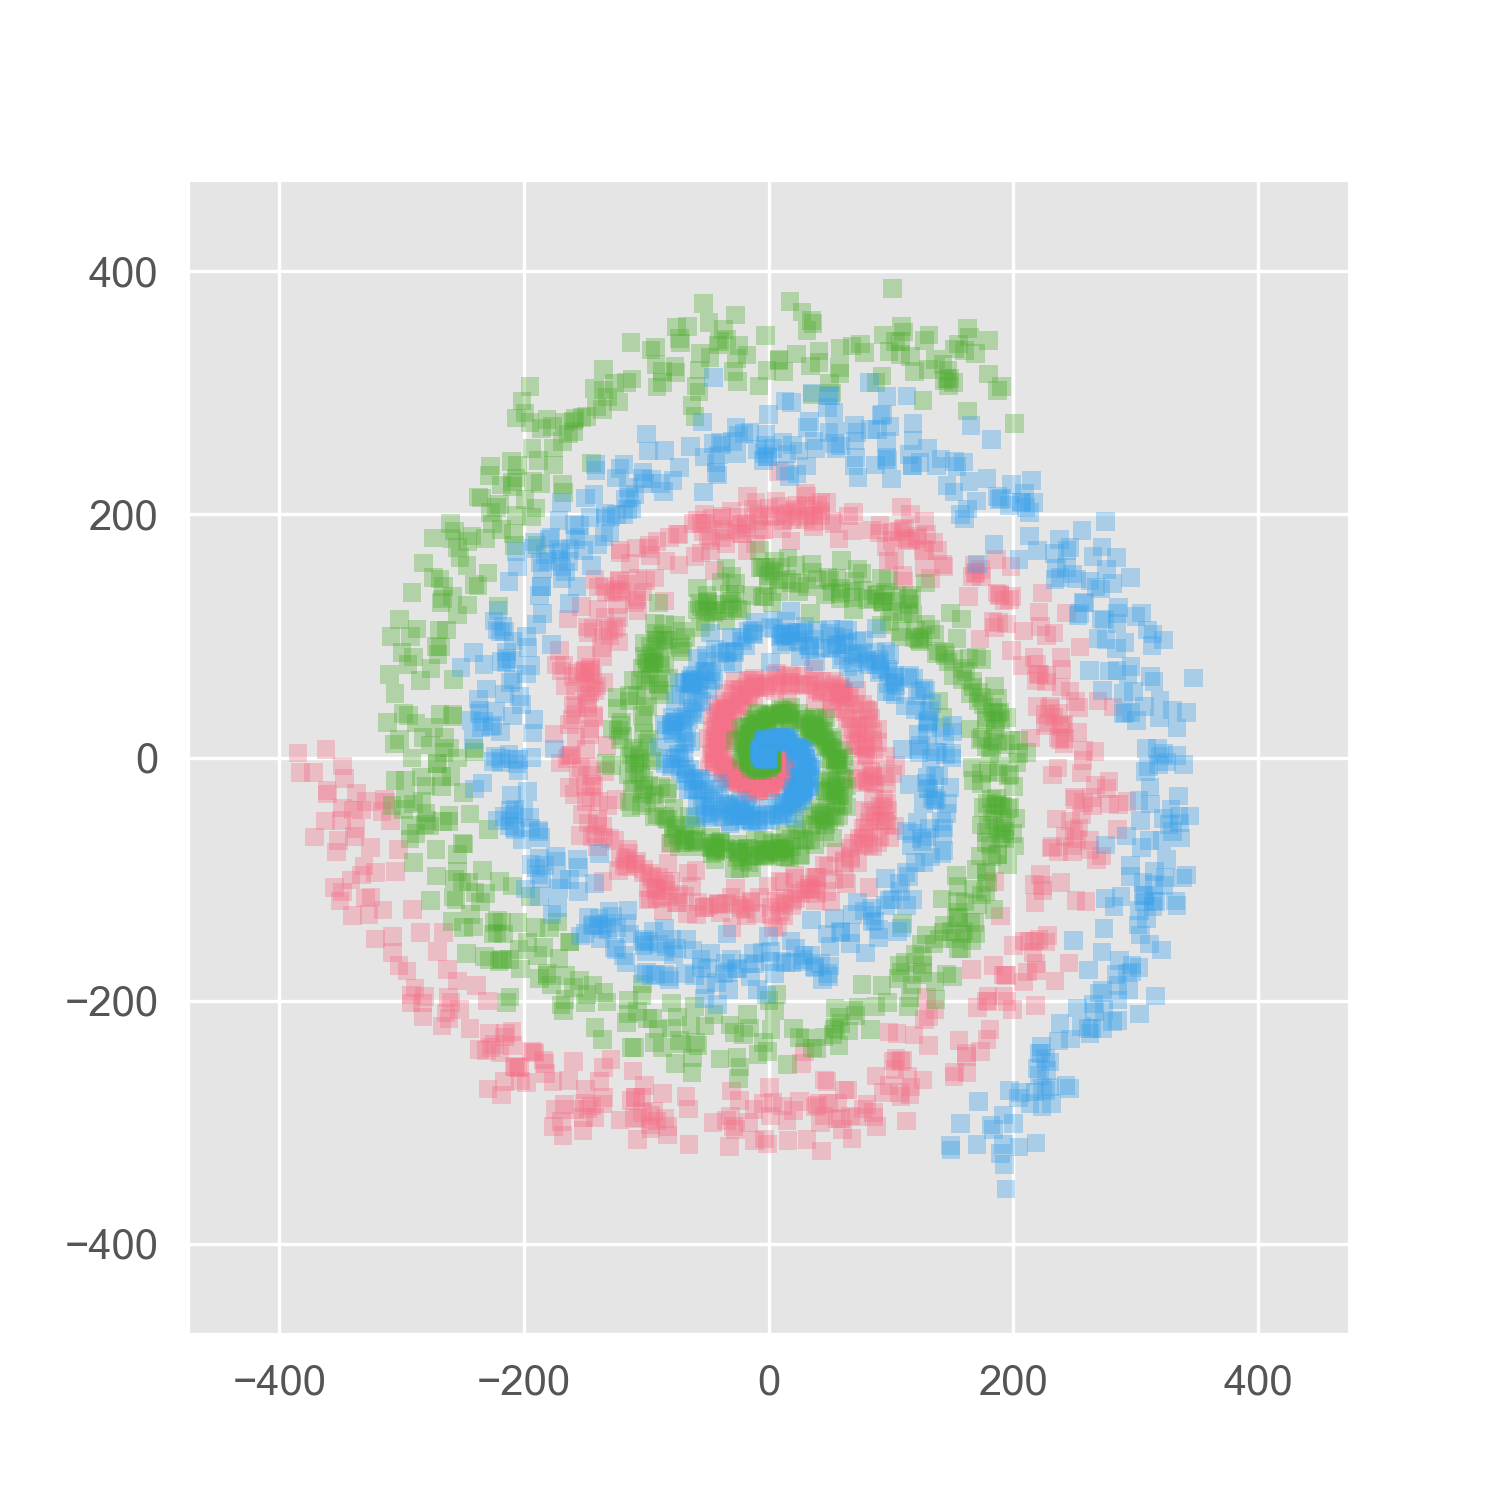
\includegraphics[trim=0 0 0 0, clip, width=\linewidth]{../openreview/plots/2a.png}
      \label{fig:2a}
    \end{subfigure}
    \begin{subfigure}{0.4\textwidth}
      \centering
      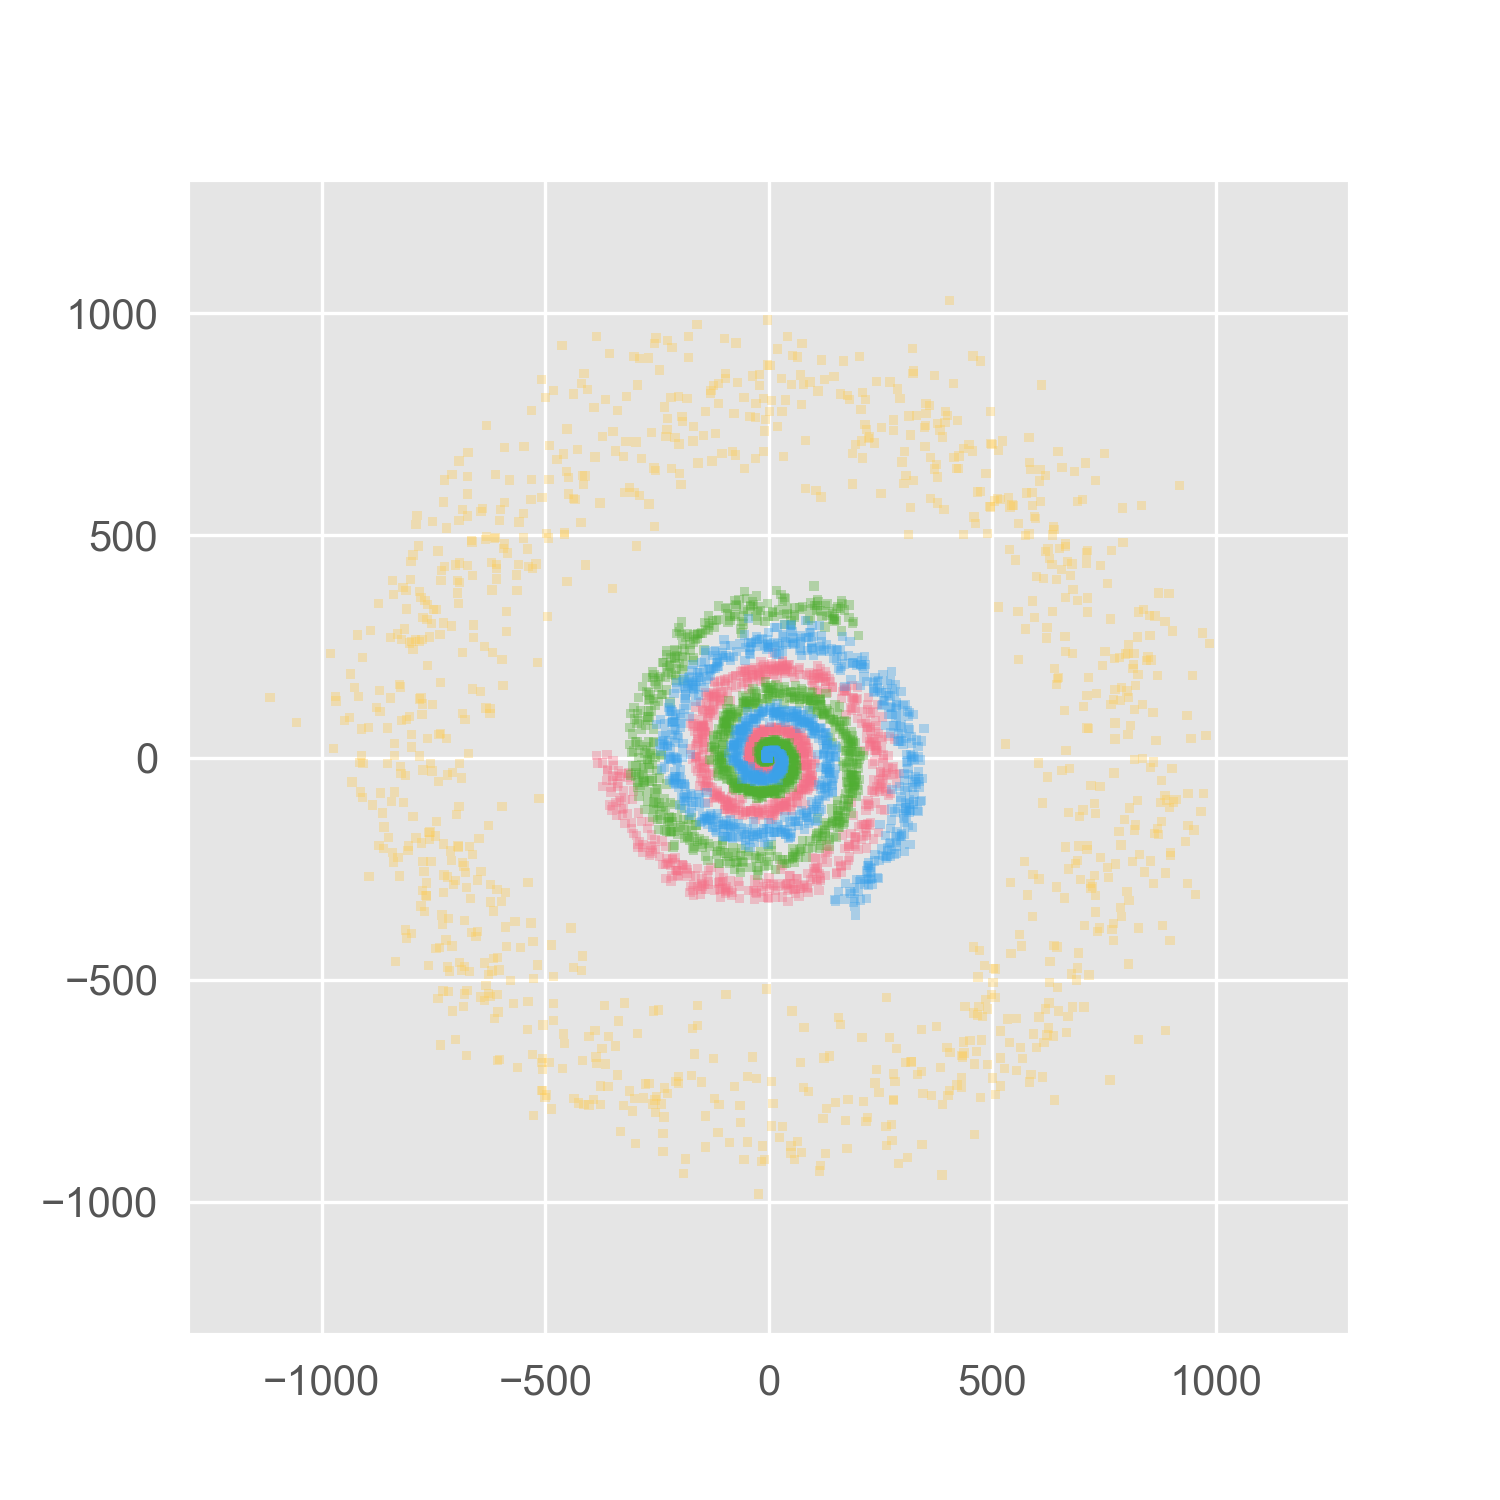
\includegraphics[trim=0 0 0 0, clip, width=\linewidth]{../openreview/plots/2b.png}
      \label{fig:2b}
    \end{subfigure}
    \caption{The synthetic, spiral dataset. }
    \label{fig:2}
\end{figure}

 

\subsubsection{Model description and hyperparameters}
The original paper does not specify what type of neural network was used for classification. We were also unable to find it in the (unofficial) code. Instead, we chose to use a simple DNN with four hidden layers, each of width 64 with ReLu-activation functions, trained by minimizing the categorical cross-entropy using the Adam-optimizer, all with standard \texttt{tf.keras} settings, for 85 epochs. EnD and \EnDD \ used the same base model but was instead trained for 500 epochs. 


\subsubsection{Experimental setup and code}

On the output of an ensemble of 100 models, all differently randomly initialized, we train EnD and EnD$^2$ both with and without auxiliary data, using an initial temperature of 1, as in the paper. Doing this, we observed that the training diverges for many initialisations, mainly for \EnDDaux. Thus, we also used an initial temperature of $T = 2.5$, both with and without annealing. The annealing schedule was $T = 2.5$ between epoch 0 and 200, linearly decreasing to 1 between epoch 200 and 400 and 1 between epoch 400 and 500. Additionally, we also trained a model EnD$^2_{\texttt{+AUX20}}$, with only 20 samples from the auxiliary dataset. 

All 7 models were trained 20 times, with different random initialisations. To make sure they converged, the test error was calculated. In cases test error was above 10\%, it was deemed as non-convergence, and not taken into account. Among the converged ones, the mean error and the 95\%-confidence interval around the mean is calculated, assuming a normal distribution. This means that for cases with fewer samples, the confidence interval is larger.  

The main goal of this experiment is to visually show the total uncertainty, the data uncertainty and the knowledge uncertainty. They were calculated as specified in \cite{malinin2019ensemble} and \cite{NIPS2018_7936}, for the grid $[-2000, 2000] \times [-2000, 2000]$ at all coordinates divisible by four, for a total of $10^6$ points. 

The full code is available at \href{https://anonymous.4open.science/r/4ee2c9ef-295f-44e2-8214-f0818b932817/}{https://anonymous.4open.science/r/4ee2c9ef-295f-44e2-8214-f0818b932817/}.


\subsubsection{Computational requirements}
The experiments were run on the CPU of a normal laptop (2.7 GHz Dual-Core i5). The total time to reproduce the ensemble of 100 models and all 20 repetitions of all 7 tested distillation methods, is around 5 to 6 hours.

\subsection{Results}


\subsubsection{Classification accuracy}
In Table \ref{tab:spiral}, the classification accuracy from our experiment and the original paper is reported. We see that 
\begin{itemize}
    \item the ensemble outperforms the individual models, and that all distillation methods perform closer to the ensemble, than an individual model.
    \item the best performance is achieved by EnD with auxiliary data. 
    \item using annealing or not when starting at $T = 2.5$ does not affect the final classification accuracy. 
\end{itemize}

 \begin{table}
\centering
\caption{Classification error on Spiral Dataset, compared with \cite{malinin2019ensemble}. Error bars are 95\%-confidence intervals assuming normal distribution. Note that our results likely use a different base model and training procedure than the original paper, since it was not specified there.  }
\addtolength{\leftskip} {-3cm}
\addtolength{\rightskip}{-3cm}
\begin{tabular}{r||r|r|r|r|r|r|r|r|r} 
\hline
\textbf{ERR$\downarrow$} & 
IND & 
ENSM & 
EnD & 
$\text{EnD}^2$ & 
EnD & 
EnD$^2$ & 
EnD$^2$ & 
EnD$^2$ & 
EnD$^2$ &  \\[-16pt]
& 
& 
& 
& 
& 
$_{\texttt{+AUX}}$ & 
$_{\texttt{+AUX}}$ & 
$_{\texttt{+AUX,ANN}}$ & 
$_{\texttt{+AUX,T=2.5}}$ & 
$_{\texttt{+AUX20}}$ &  %[0.5ex]
\hline
\hline
Our results & 
8.20$\scriptstyle \pm 0.67$ &
2.3$\scriptstyle \pm NA$ &
3.90$\scriptstyle \pm 0.65$&
3.86$\scriptstyle \pm 0.70$&
2.61$\scriptstyle \pm 0.11$&
4.67$\scriptstyle \pm 3.26$&
3.30$\scriptstyle \pm 0.59$&
3.45$\scriptstyle \pm 0.96$&
5.0$\scriptstyle \pm 1.54$ \\ 
Paper \cite{malinin2019ensemble} &
13.21 &
12.37 &
12.39 &
12.47 &
12.41 &
12.40 &
- &
- &
-\\ 
\hline
\end{tabular}
\\ [1ex] 

\label{tab:spiral}
\end{table}

\subsubsection{Visualization of uncertainty}
The total, data and knowledge uncertainty is plotted in Figure \ref{fig:fig3} for a grid of 10$^6$ points. In contrast to the original paper, we fix the scale of the colour bar for better comparability between plots.

We observe that
\begin{itemize}
    \item \EnDD \ is not able to emulate the uncertainty landscape of the ensemble, but \EnDDaux \ can approximate it fairly well.
    \item Starting at a higher temperature ($T = 2.5$) and using annealing produces similar results as starting at temperature 1, but starting at temperature 2.5 and keeping it there for the entire training duration does not capture the true uncertainty. 
    \item Using a smaller auxiliary dataset gives a worse approximation of the ensemble's uncertainty landscape. 
\end{itemize}


%% Our figure 3
\begin{figure}
\centering
\begin{subfigure}{0.22\textwidth}
  \centering
  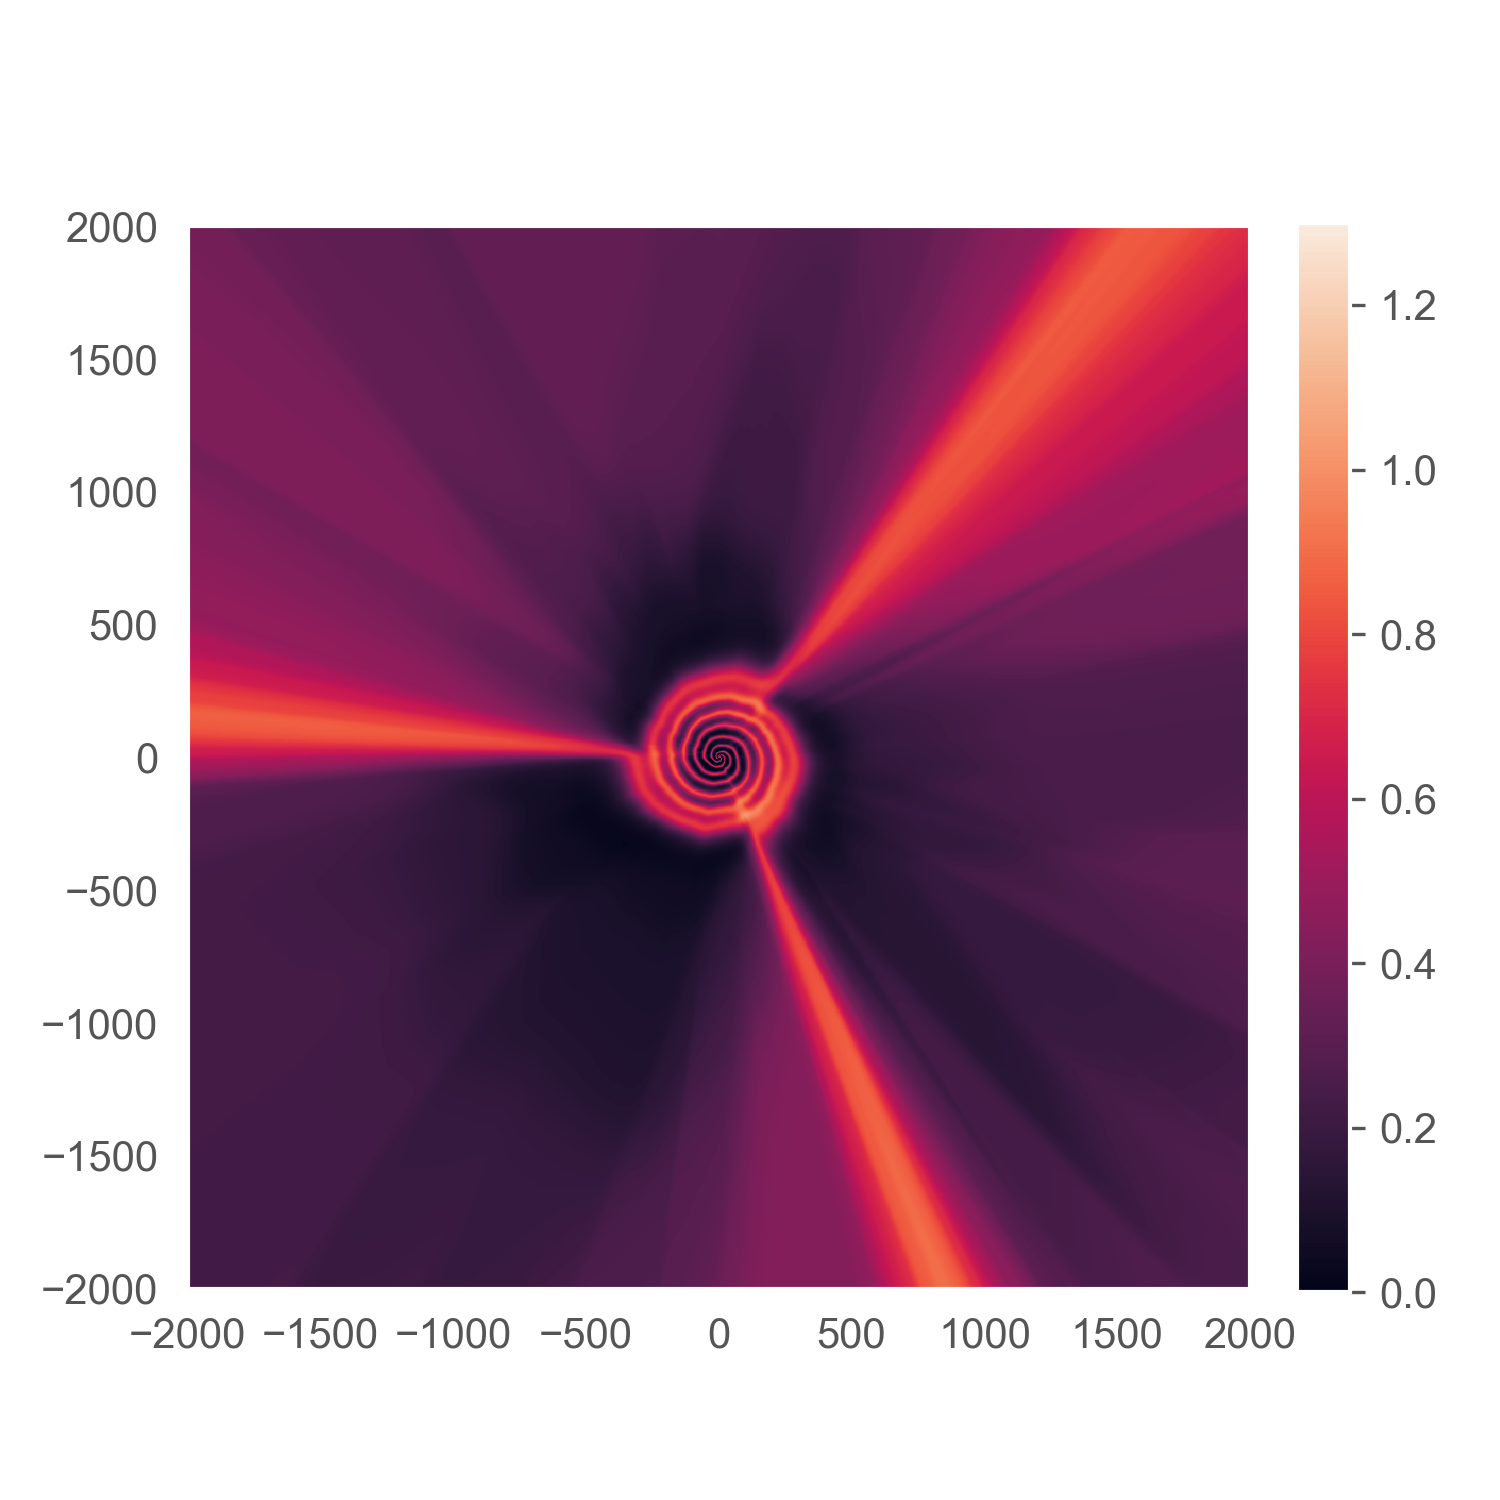
\includegraphics[trim=42 45 15 55, clip, width=\linewidth]{../openreview/plots/3a.png}
  \caption{Ensm. Tot. Unct.}
  \label{fig:3a}
\end{subfigure}
\begin{subfigure}{0.22\textwidth}
  \centering
  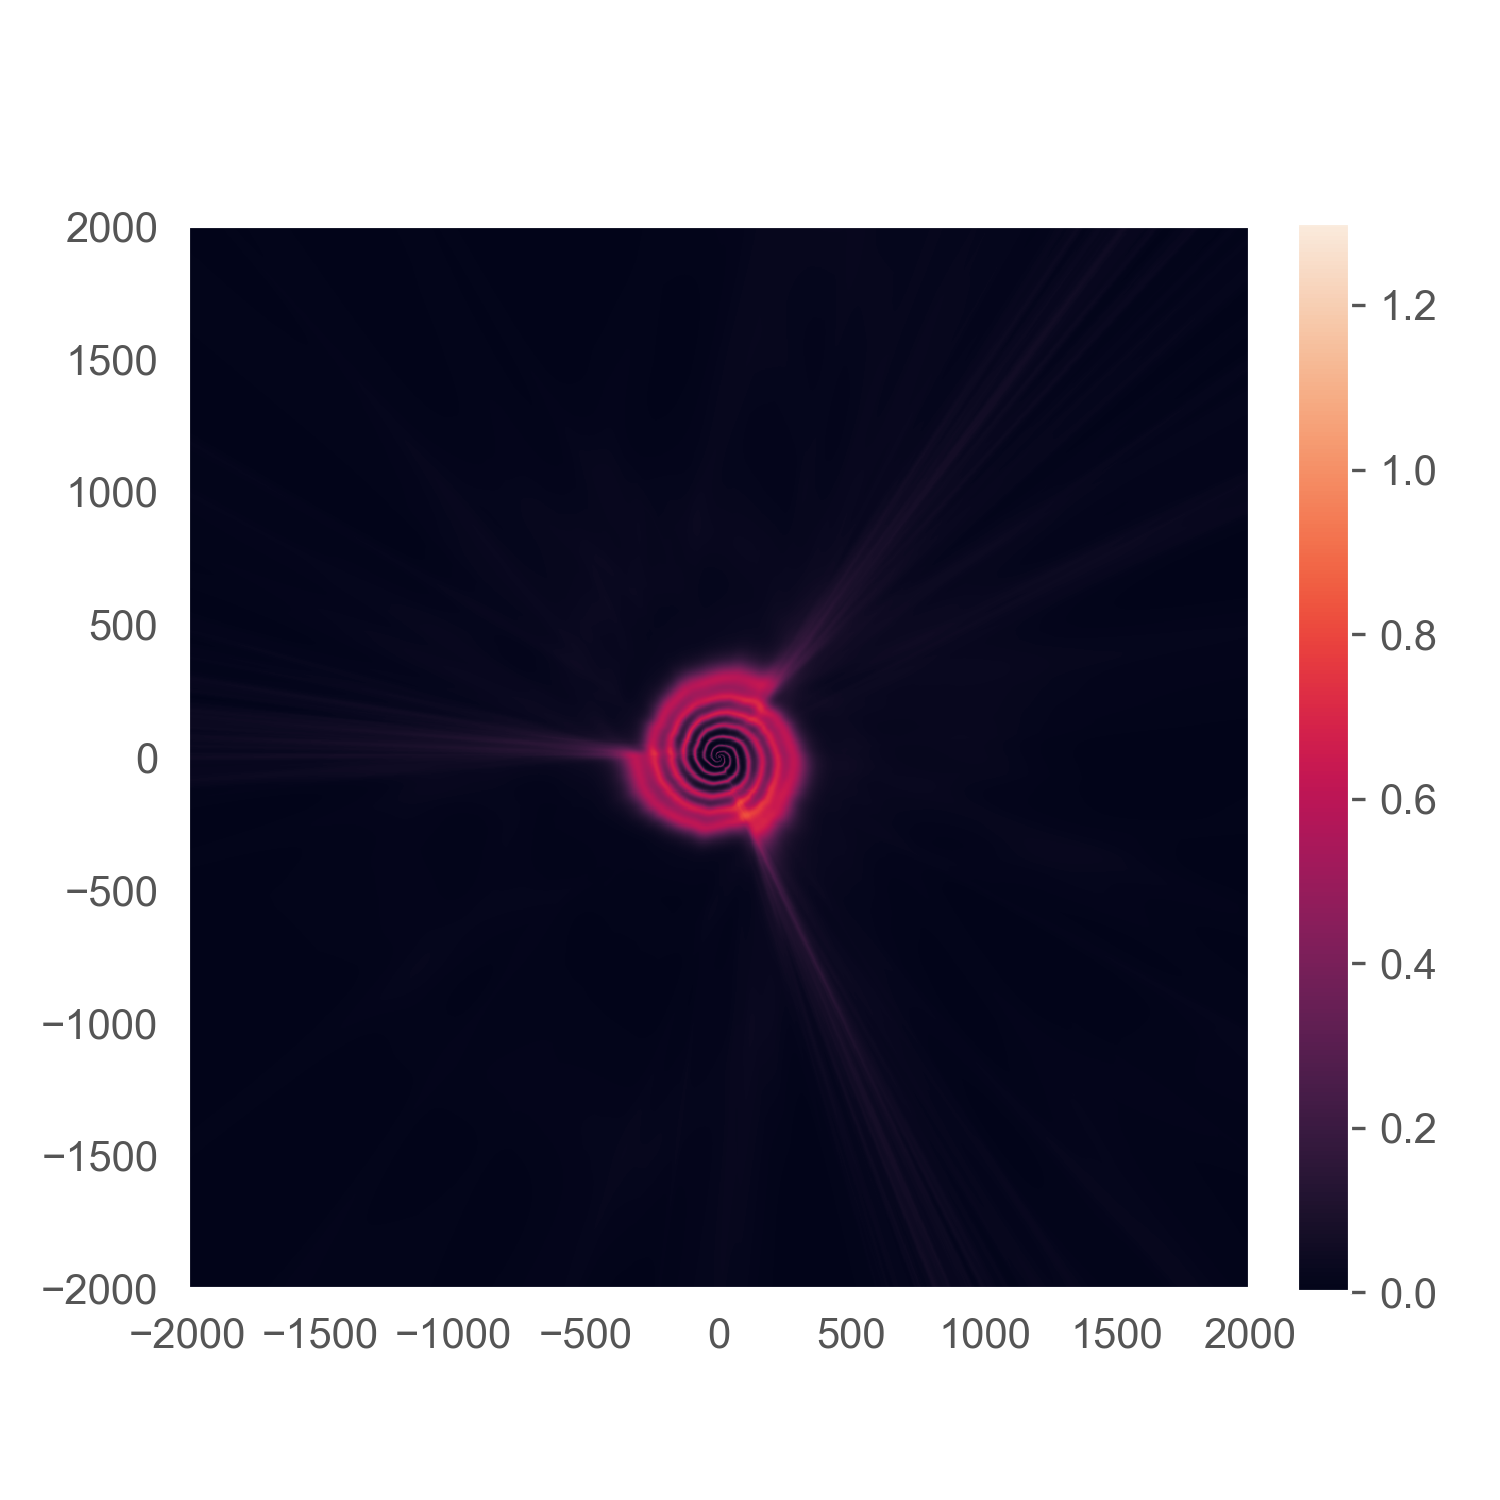
\includegraphics[trim=42 45 15 55, clip, width=\linewidth]{../openreview/plots/3b.png}
  \caption{Ensm. Data Unct.}
  \label{fig:3b}
\end{subfigure}
\begin{subfigure}{0.22\textwidth}
  \centering
  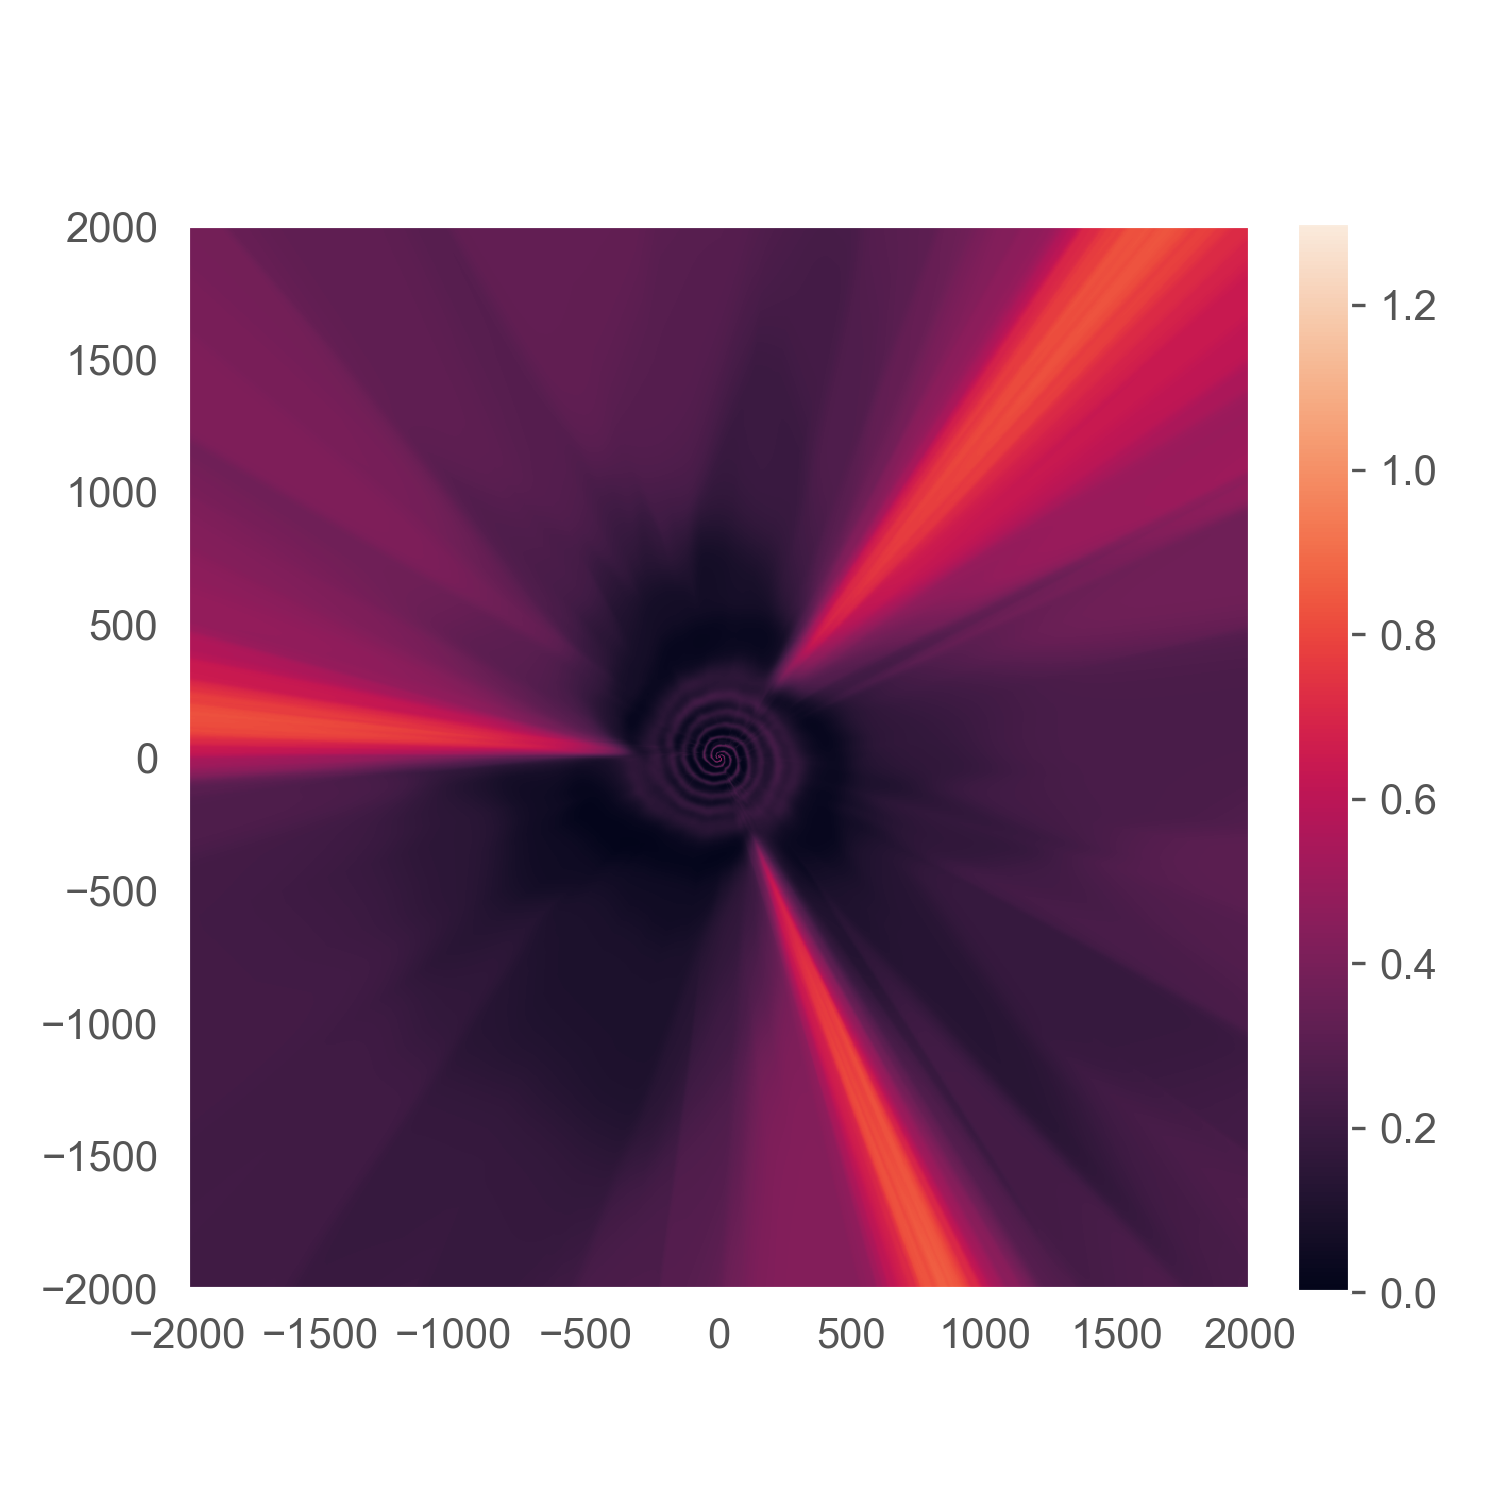
\includegraphics[trim=42 45 15 55, clip, width=\linewidth]{../openreview/plots/3c.png}
  \caption{Ensm. Know. Unct.}
  \label{fig:3c}
\end{subfigure}%

\begin{subfigure}{0.22\textwidth}
  \centering
  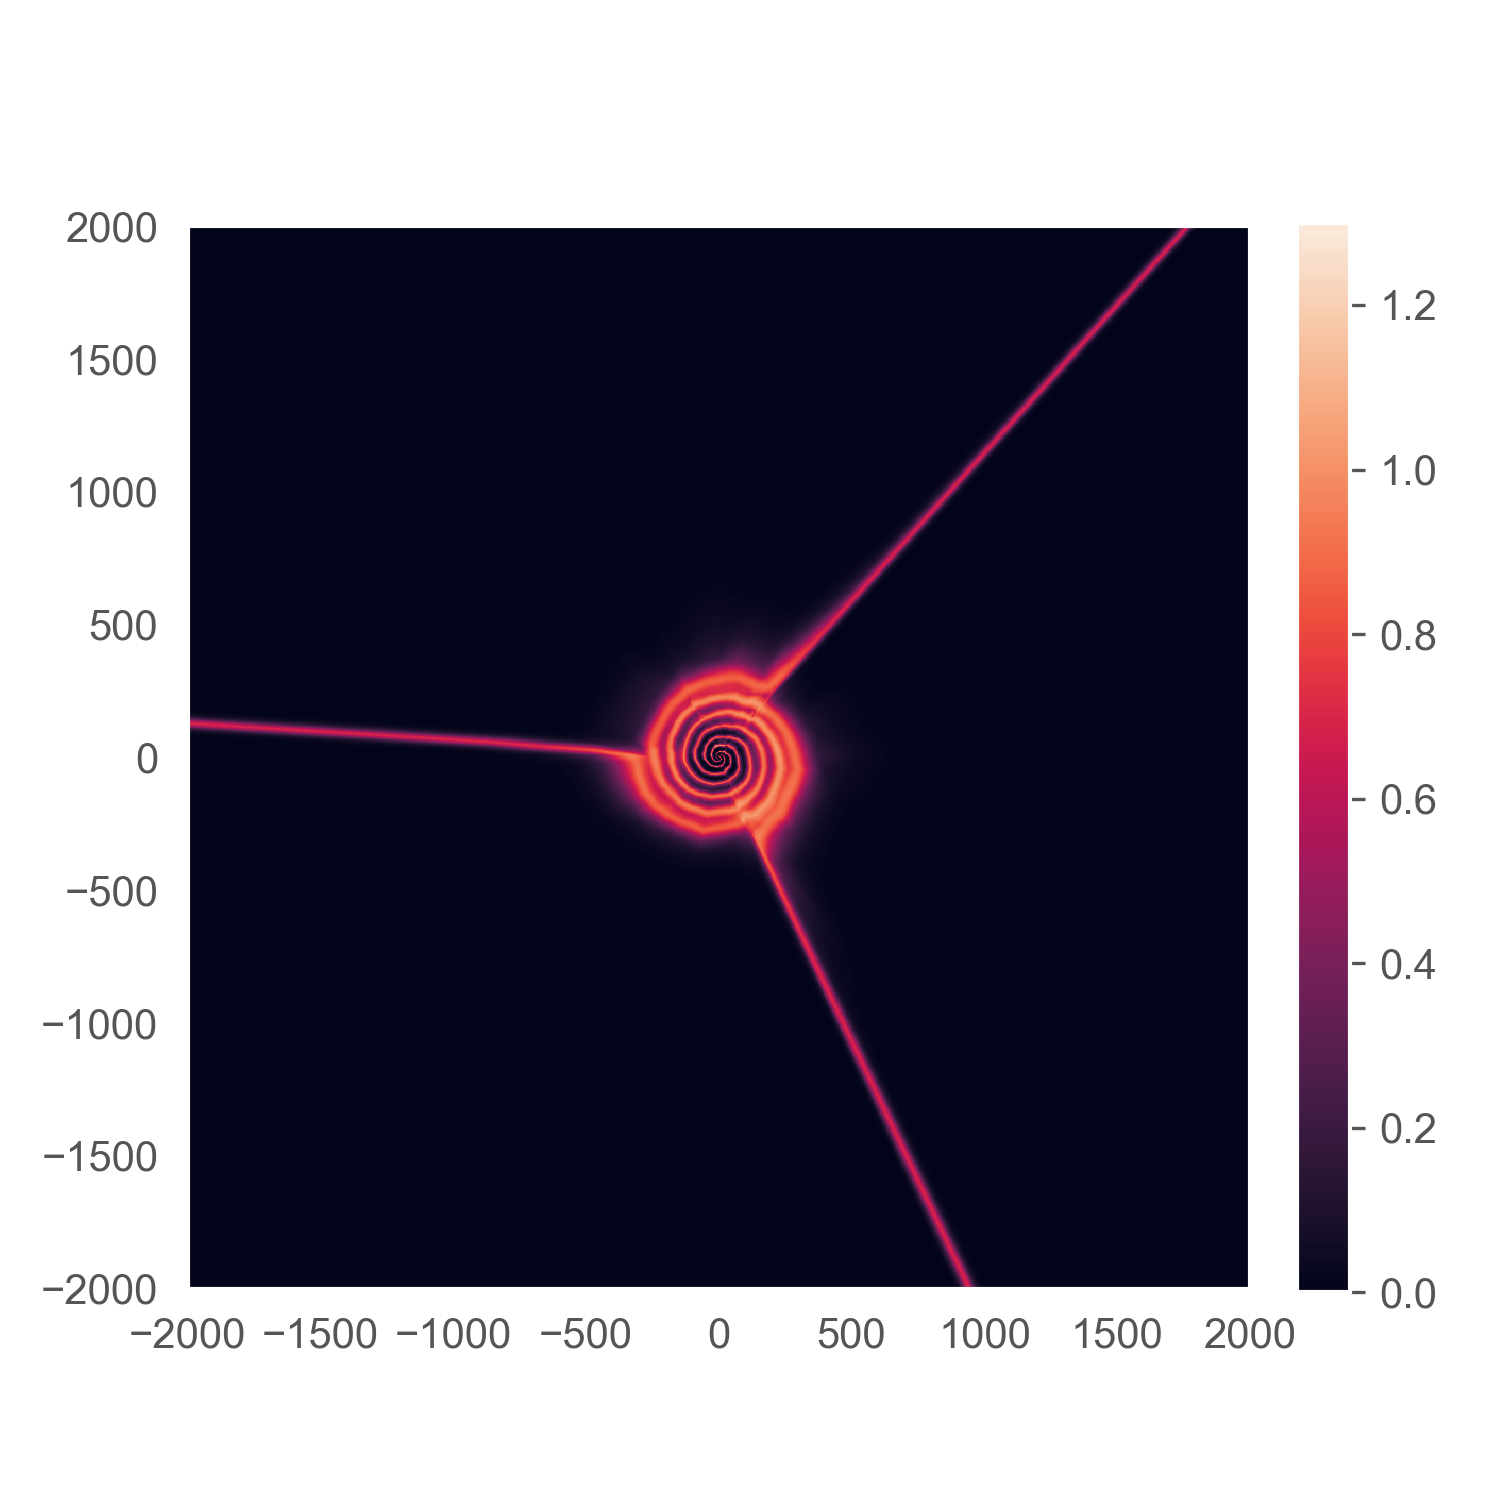
\includegraphics[trim=42 45 15 55, clip, width=\linewidth]{../openreview/plots/3d.png}
  \caption{EnD$^2$ Tot Unct.}
  \label{fig:3d}
\end{subfigure}%
\begin{subfigure}{0.22\textwidth}
  \centering
  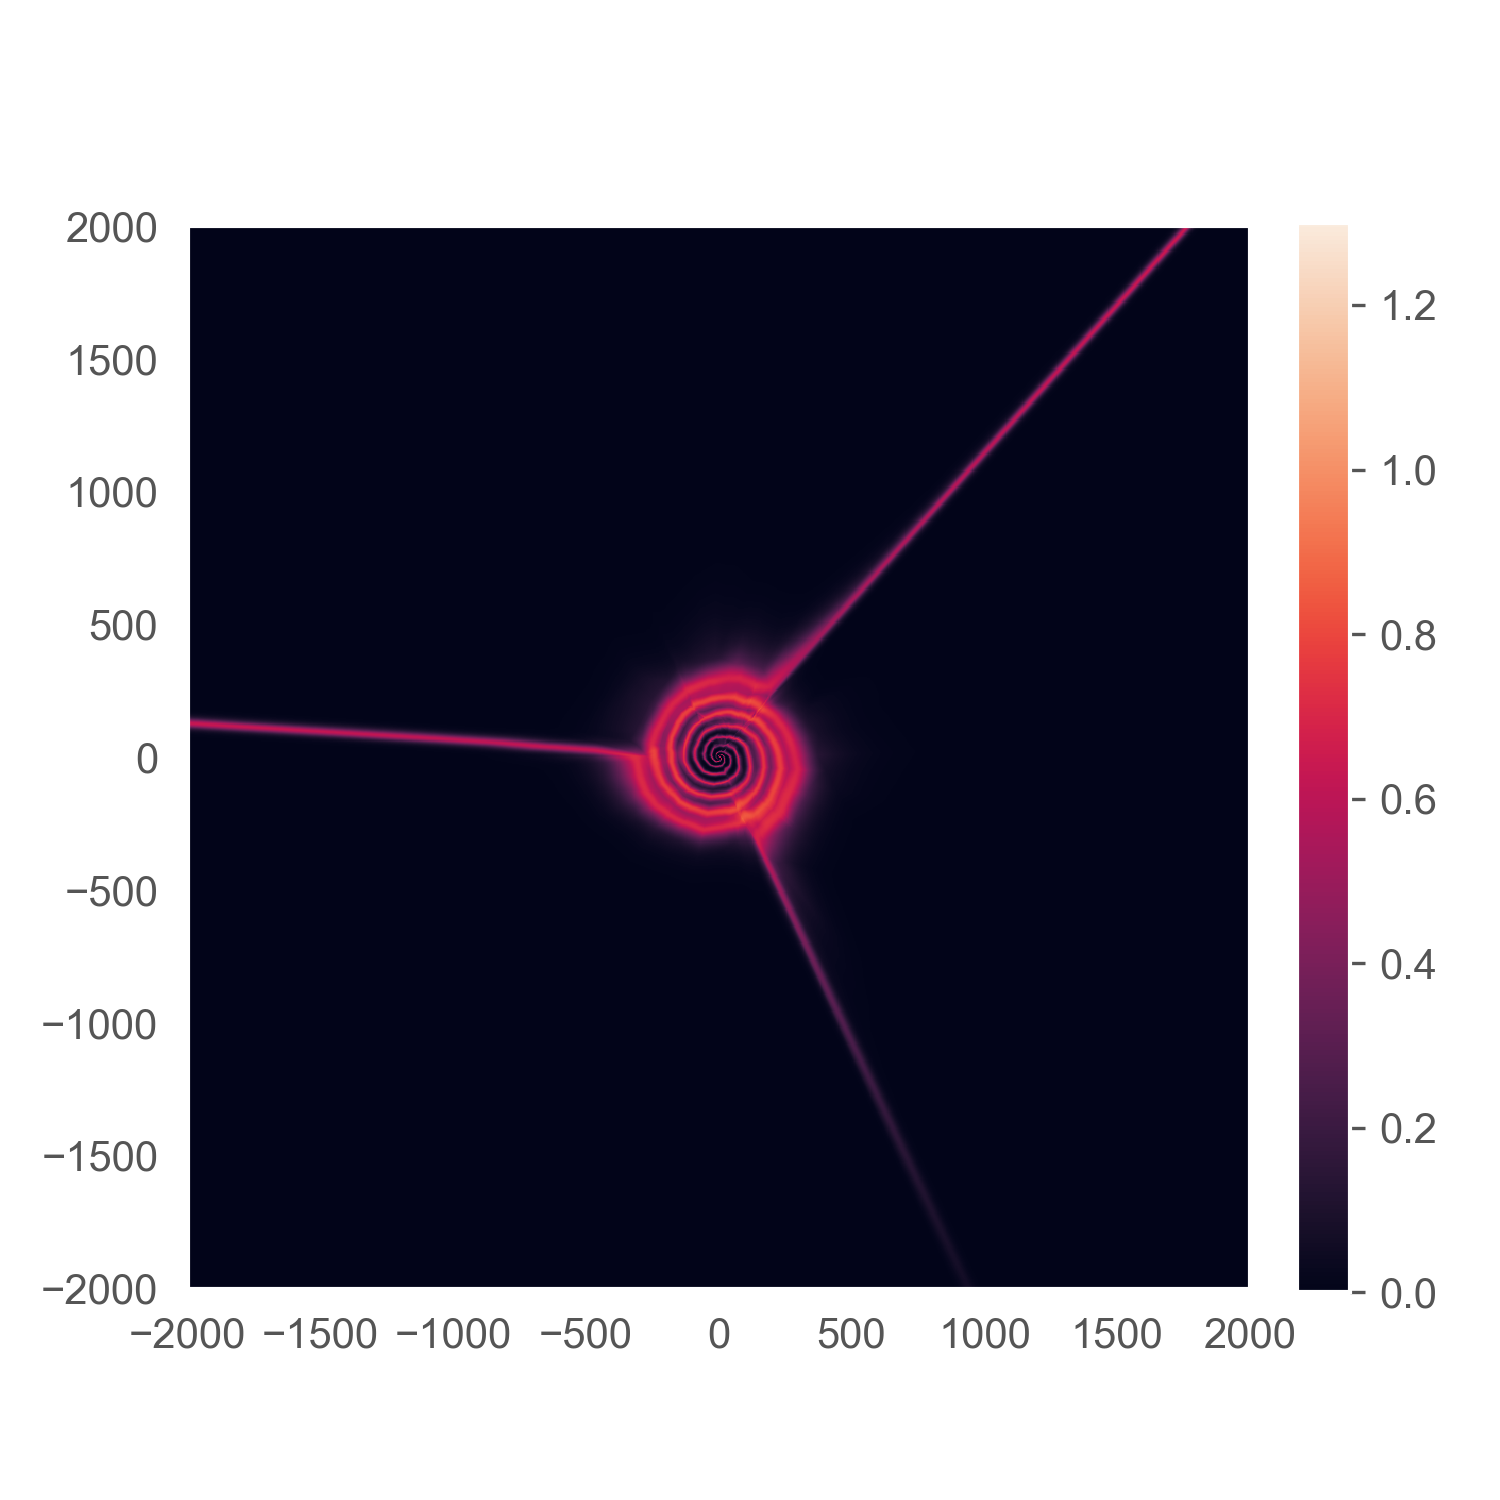
\includegraphics[trim=42 45 15 55, clip, width=\linewidth]{../openreview/plots/3e.png}
  \caption{EnD$^2$ Data Unct.}
  \label{fig:3e}
\end{subfigure}%
\begin{subfigure}{0.22\textwidth}
  \centering
  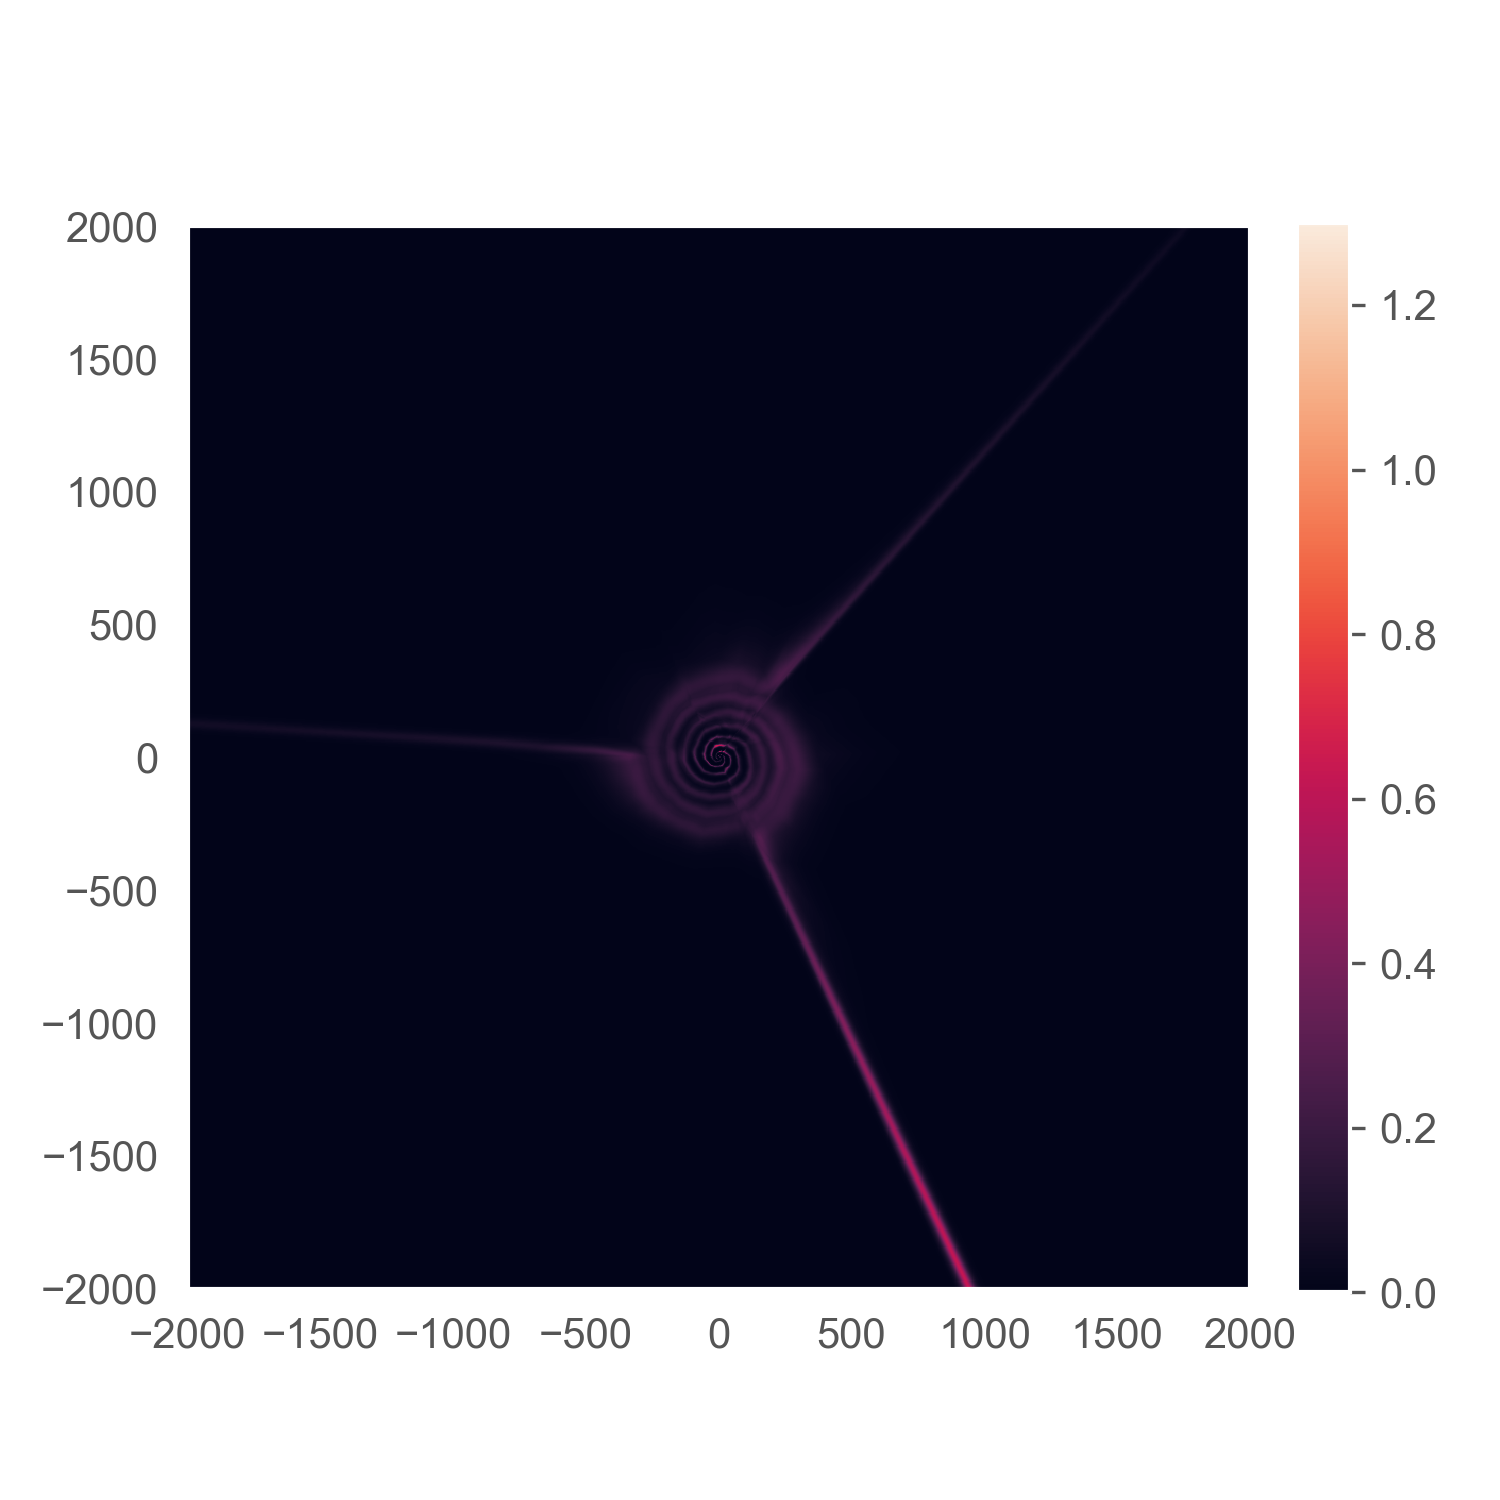
\includegraphics[trim=42 45 15 55, clip, width=\linewidth]{../openreview/plots/3f.png}
  \caption{EnD$^2$ Know. Unct.}
  \label{fig:3f}
\end{subfigure}%

\begin{subfigure}{0.22\textwidth}
  \centering
  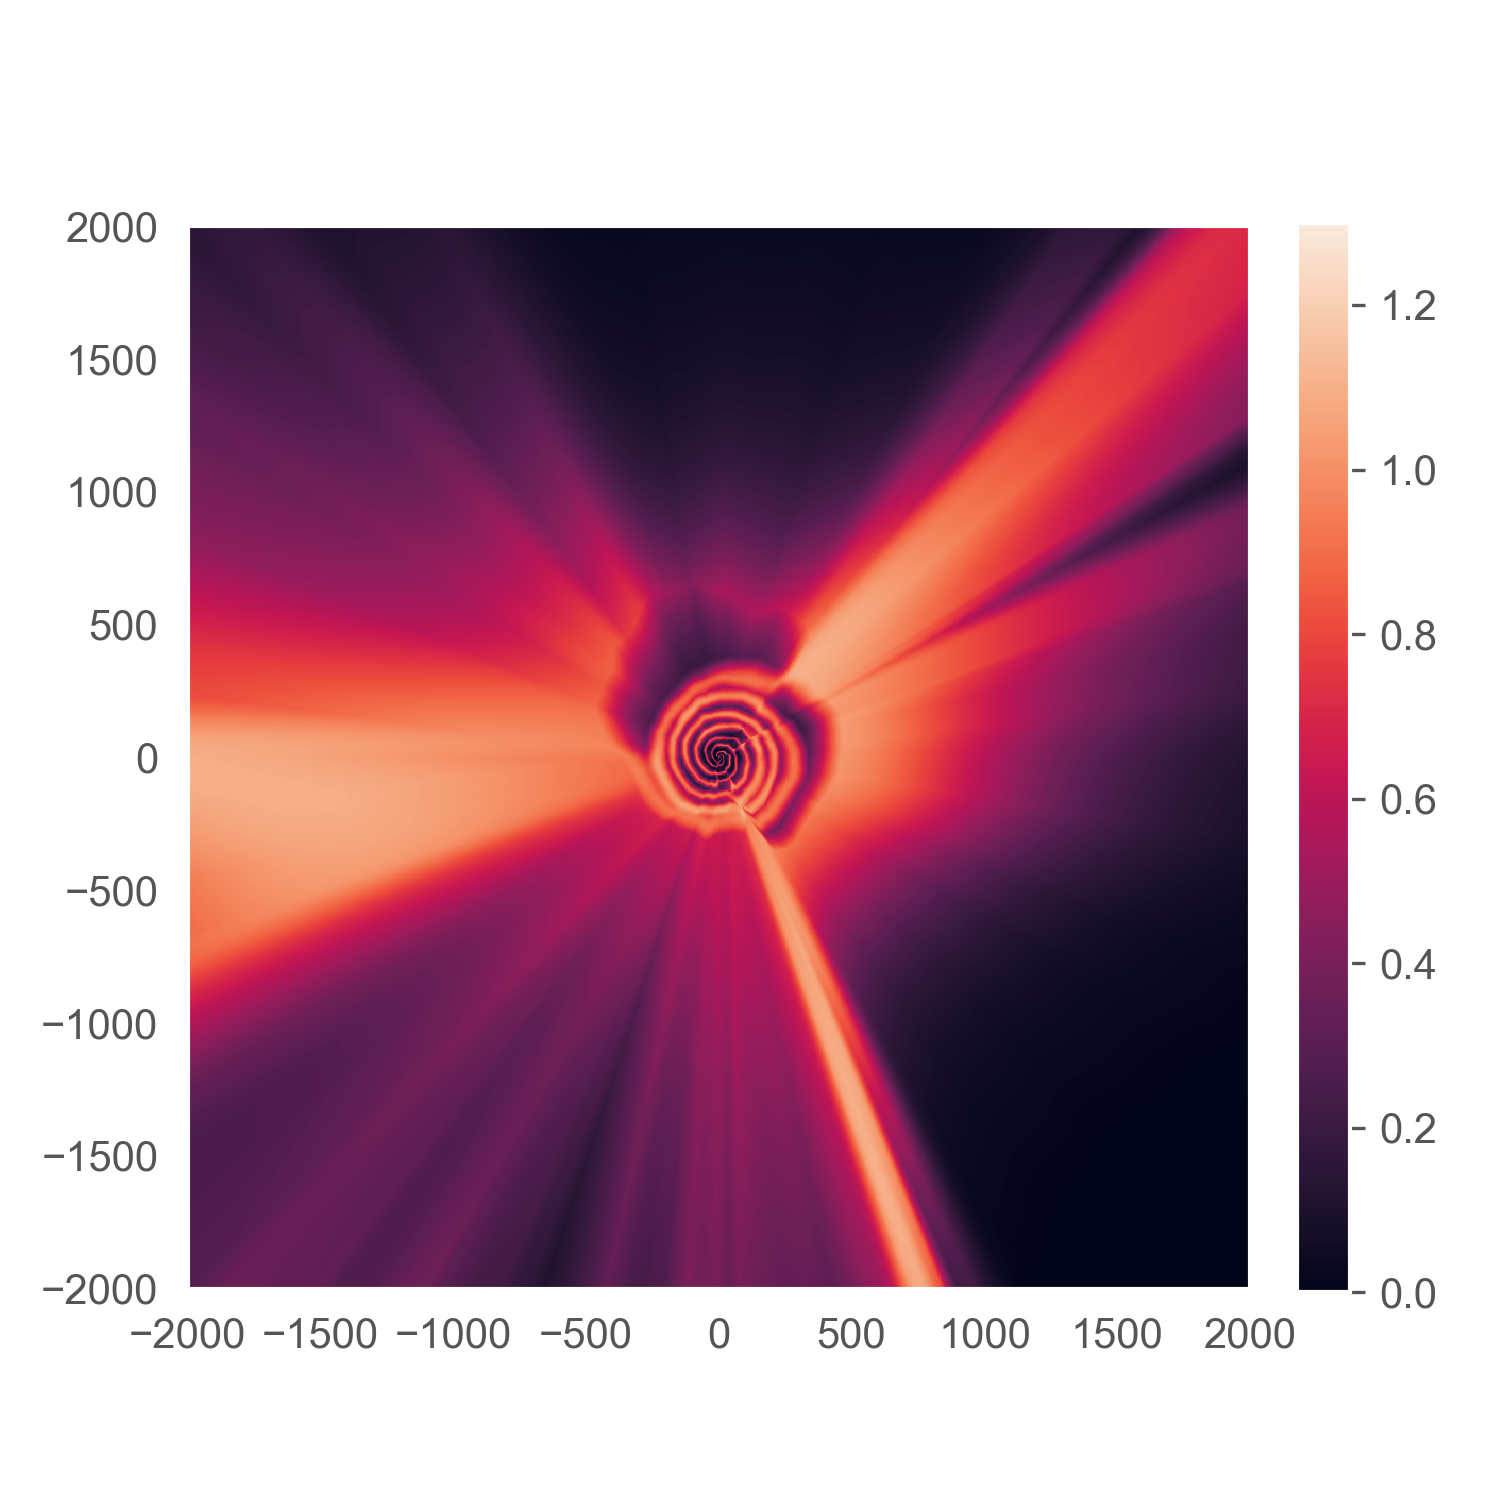
\includegraphics[trim=42 45 15 55, clip, width=\linewidth]{../openreview/plots/3g.png}
  \caption{EnD$^2_{\texttt{+AUX}}$ Tot Unct.}
  \label{fig:3g}
\end{subfigure}%
\begin{subfigure}{0.22\textwidth}
  \centering
  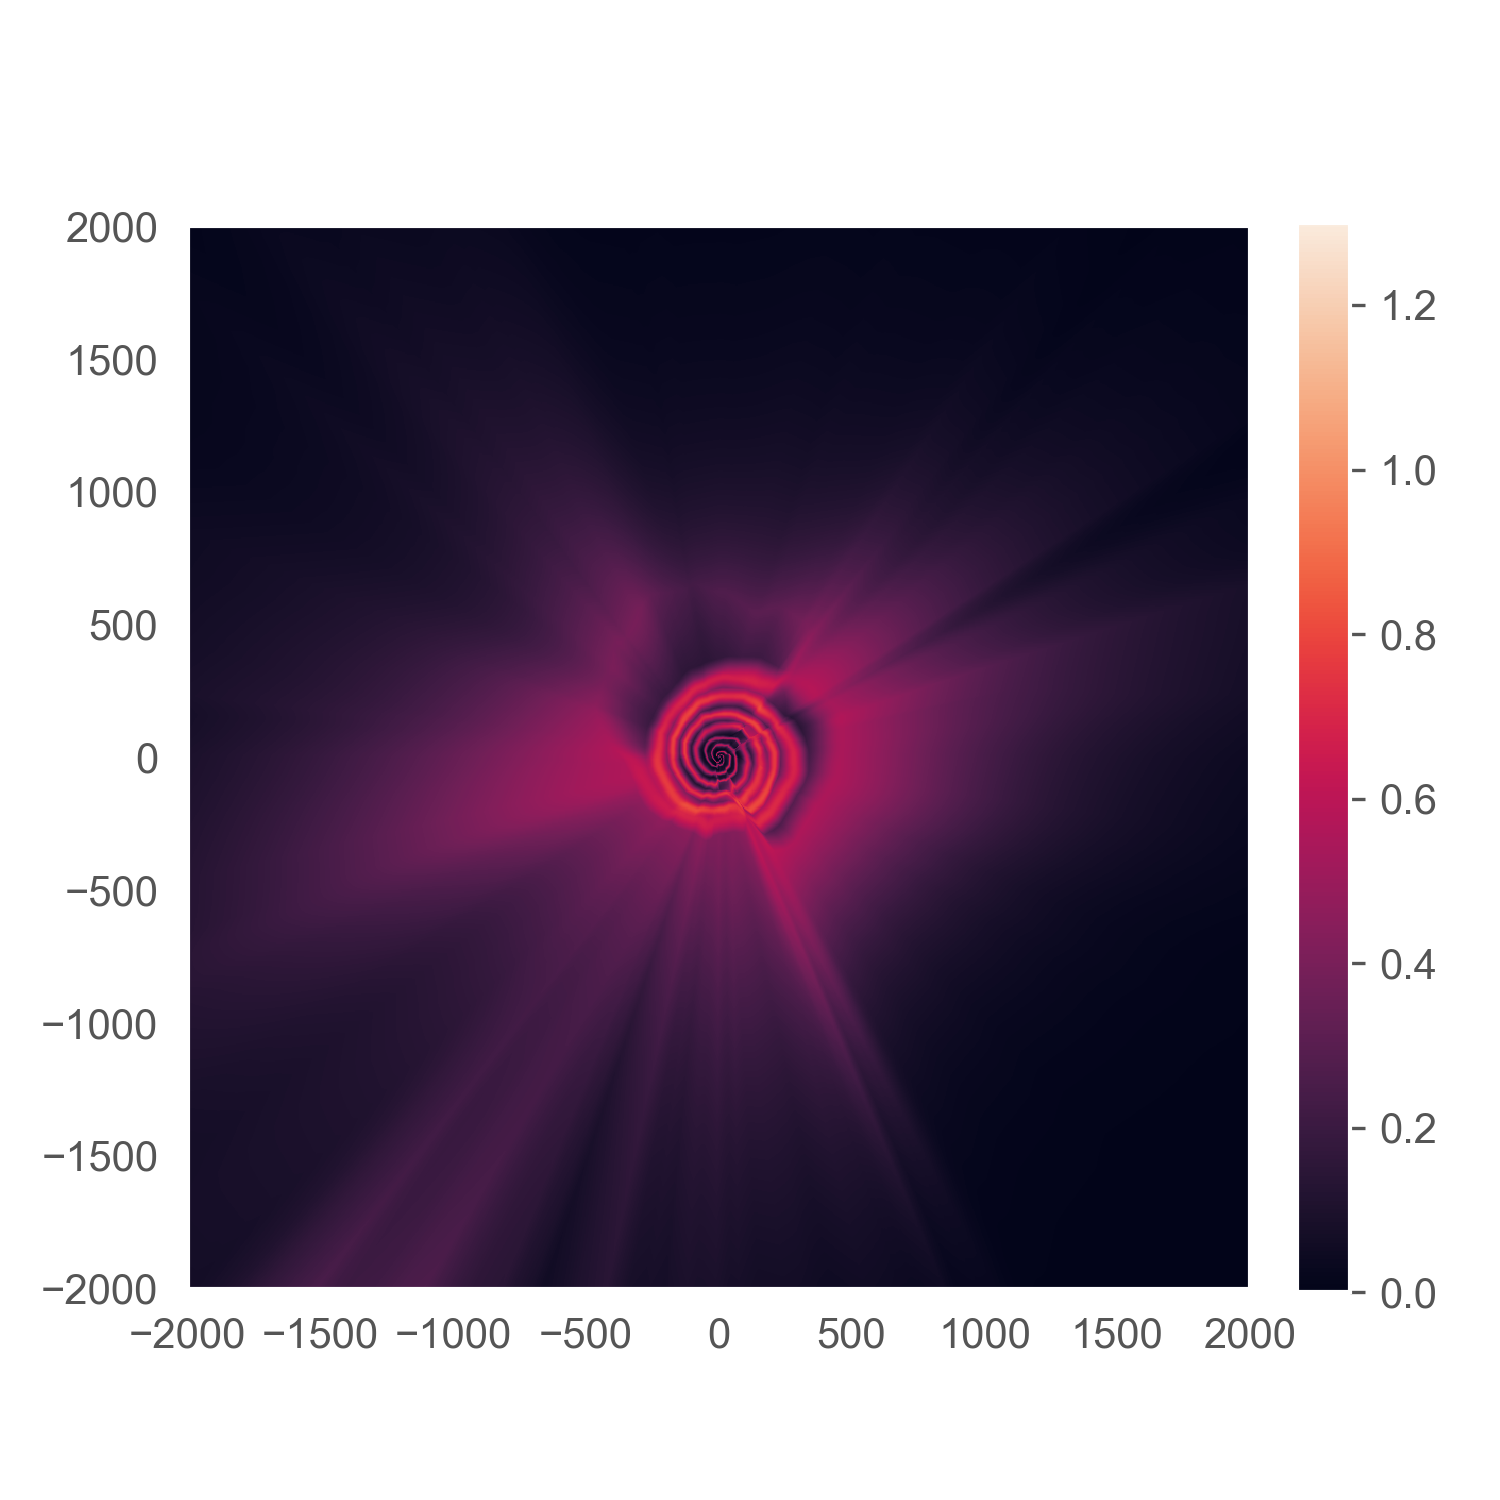
\includegraphics[trim=42 45 15 55, clip, width=\linewidth]{../openreview/plots/3h.png}
  \caption{EnD$^2_{\texttt{+AUX}}$ Data Unct.}
  \label{fig:3h}
\end{subfigure}%
\begin{subfigure}{0.22\textwidth}
  \centering
  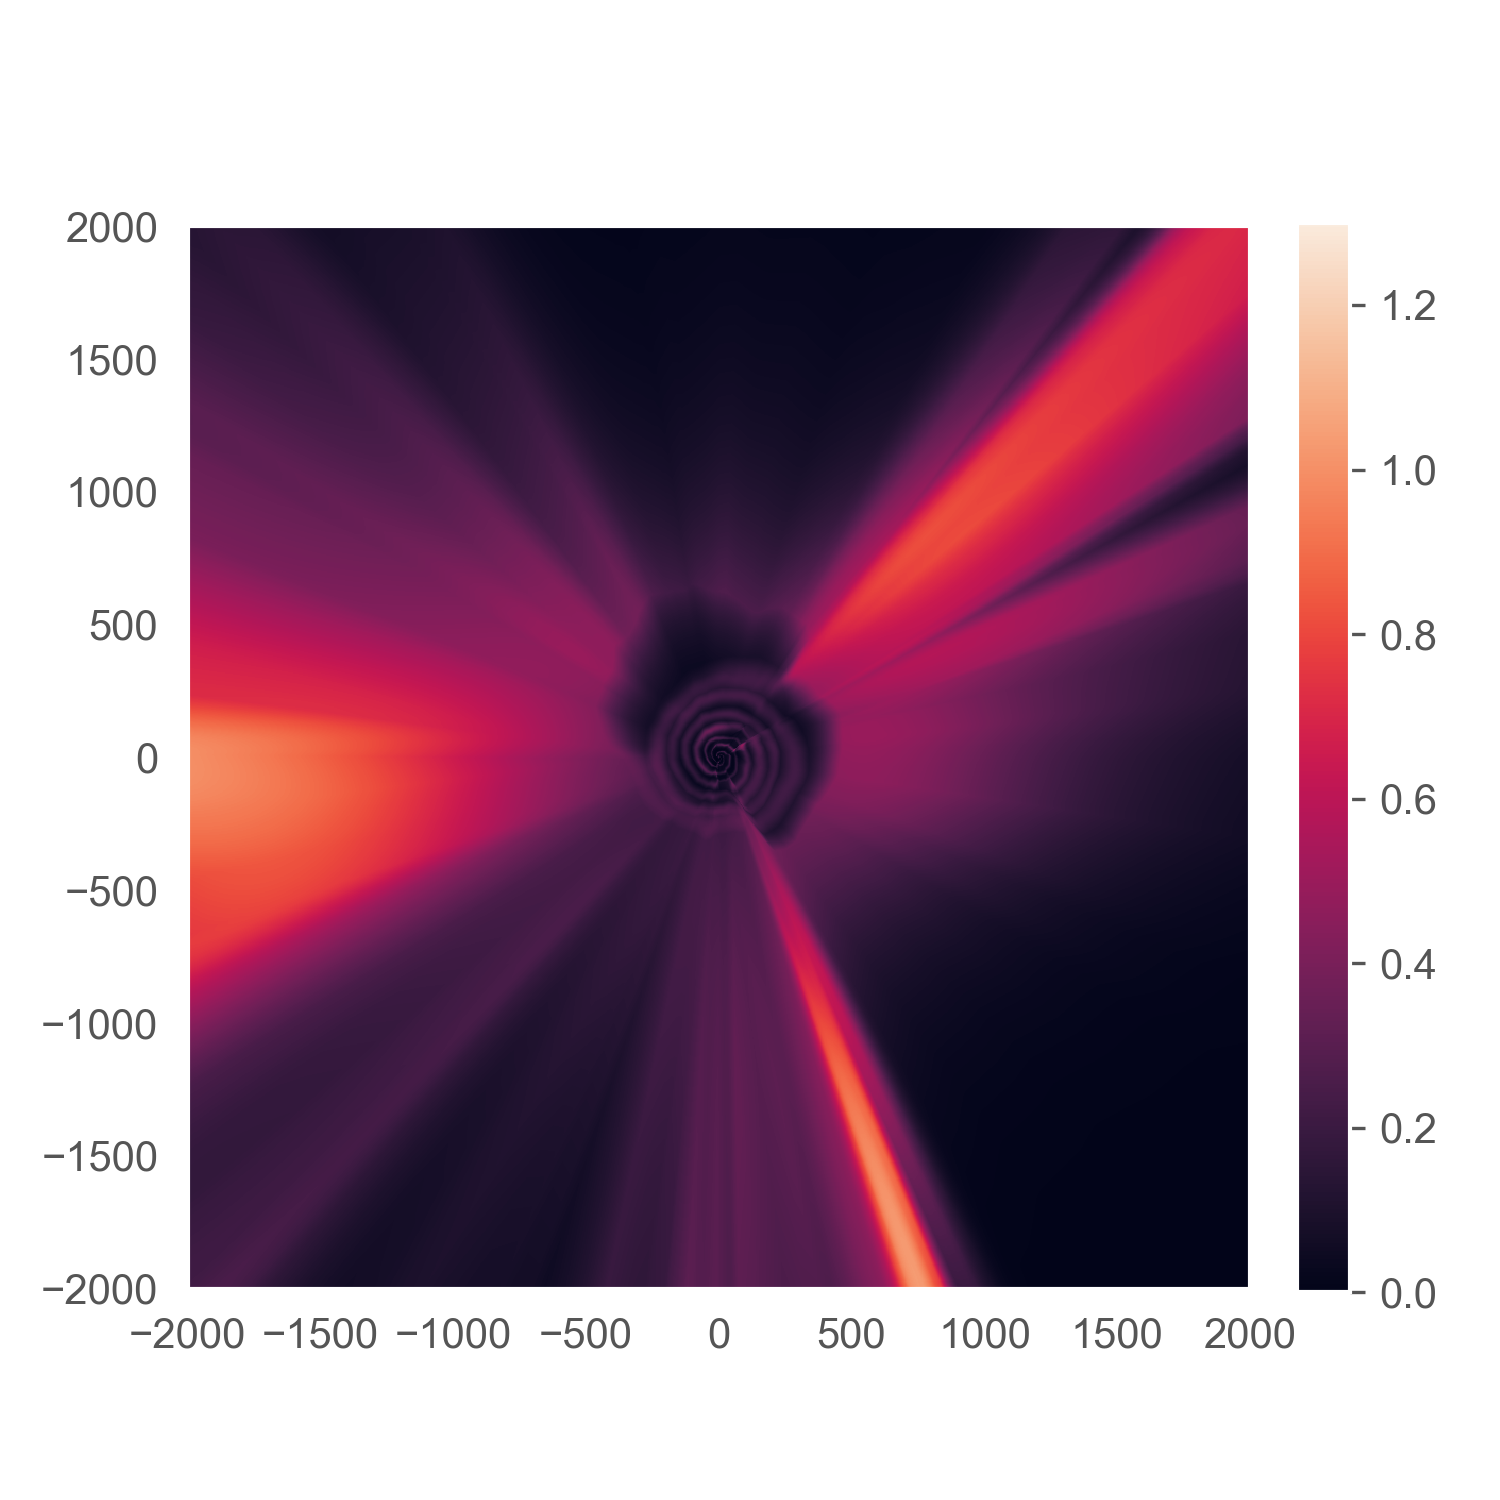
\includegraphics[trim=42 45 15 55, clip, width=\linewidth]{../openreview/plots/3i.png}
  \caption{EnD$^2_{\texttt{+AUX}}$ Know. Unct.}
  \label{fig:3i}
\end{subfigure}%

\begin{subfigure}{0.22\textwidth}
  \centering
  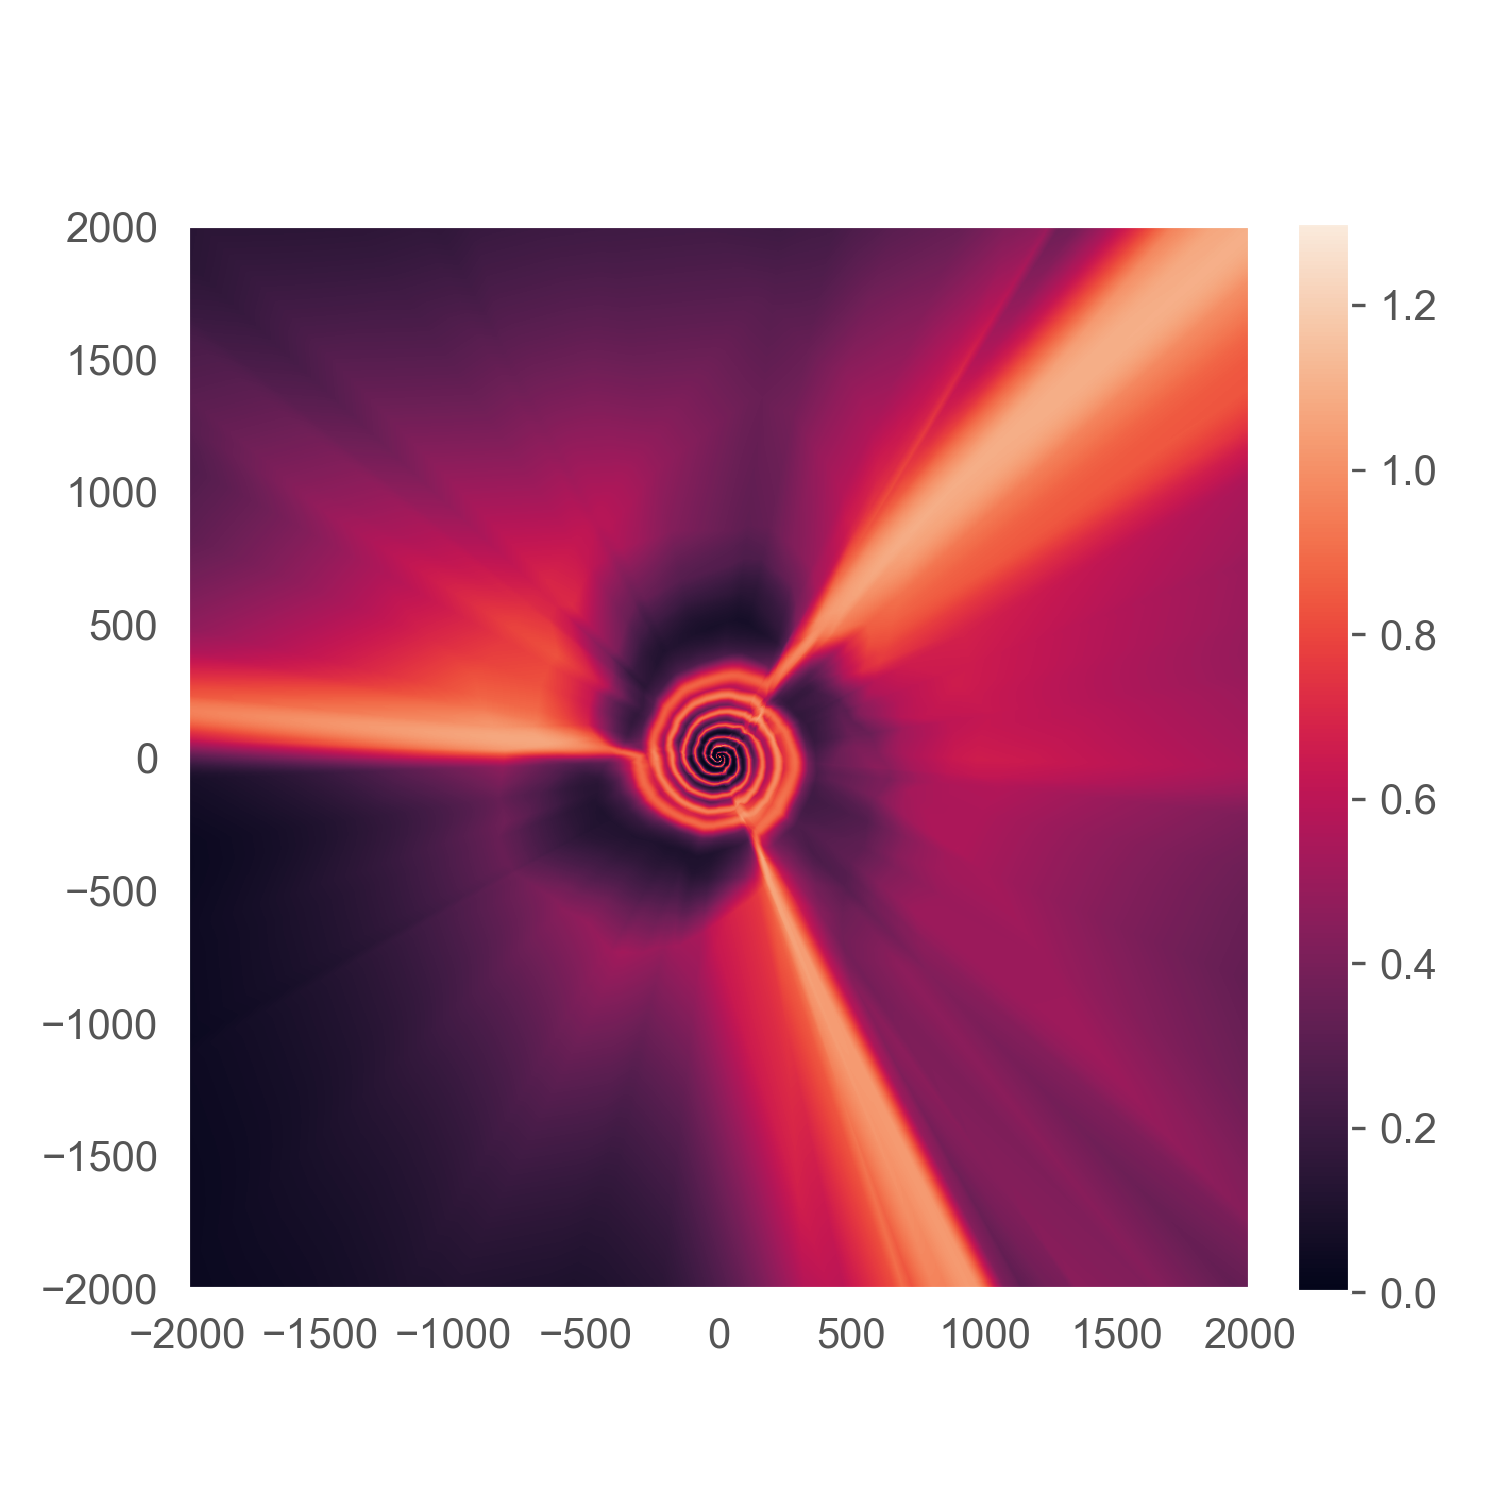
\includegraphics[trim=42 45 15 55, clip, width=\linewidth]{../openreview/plots/3j.png}
  \caption{EnD$^2_{\texttt{+AUX,ANN}}$ Total Unct.}
  \label{fig:3g}
\end{subfigure}%
\begin{subfigure}{0.22\textwidth}
  \centering
  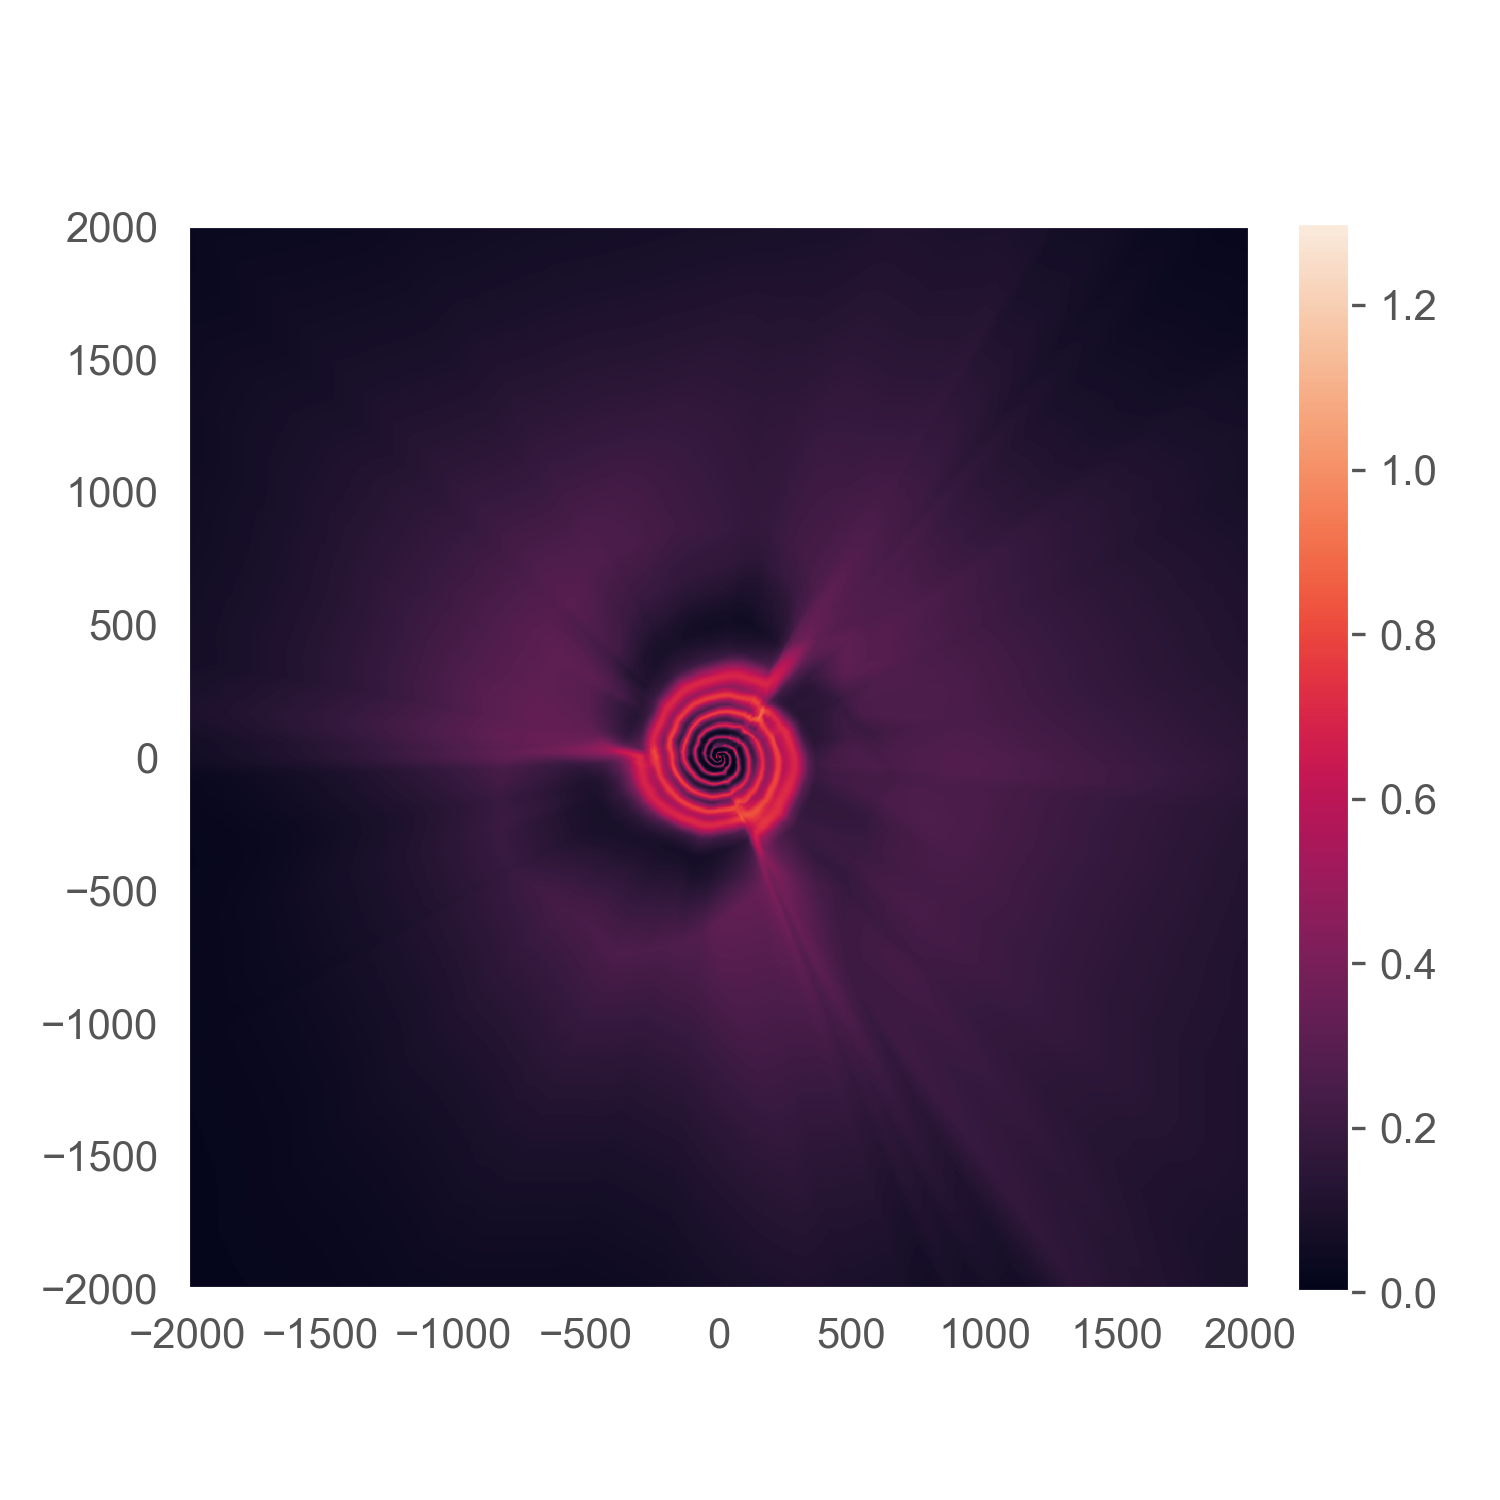
\includegraphics[trim=42 45 15 55, clip, width=\linewidth]{../openreview/plots/3k.png}
  \caption{EnD$^2_{\texttt{+AUX,ANN}}$ Data Unct.}
  \label{fig:3h}
\end{subfigure}%
\begin{subfigure}{0.22\textwidth}
  \centering
  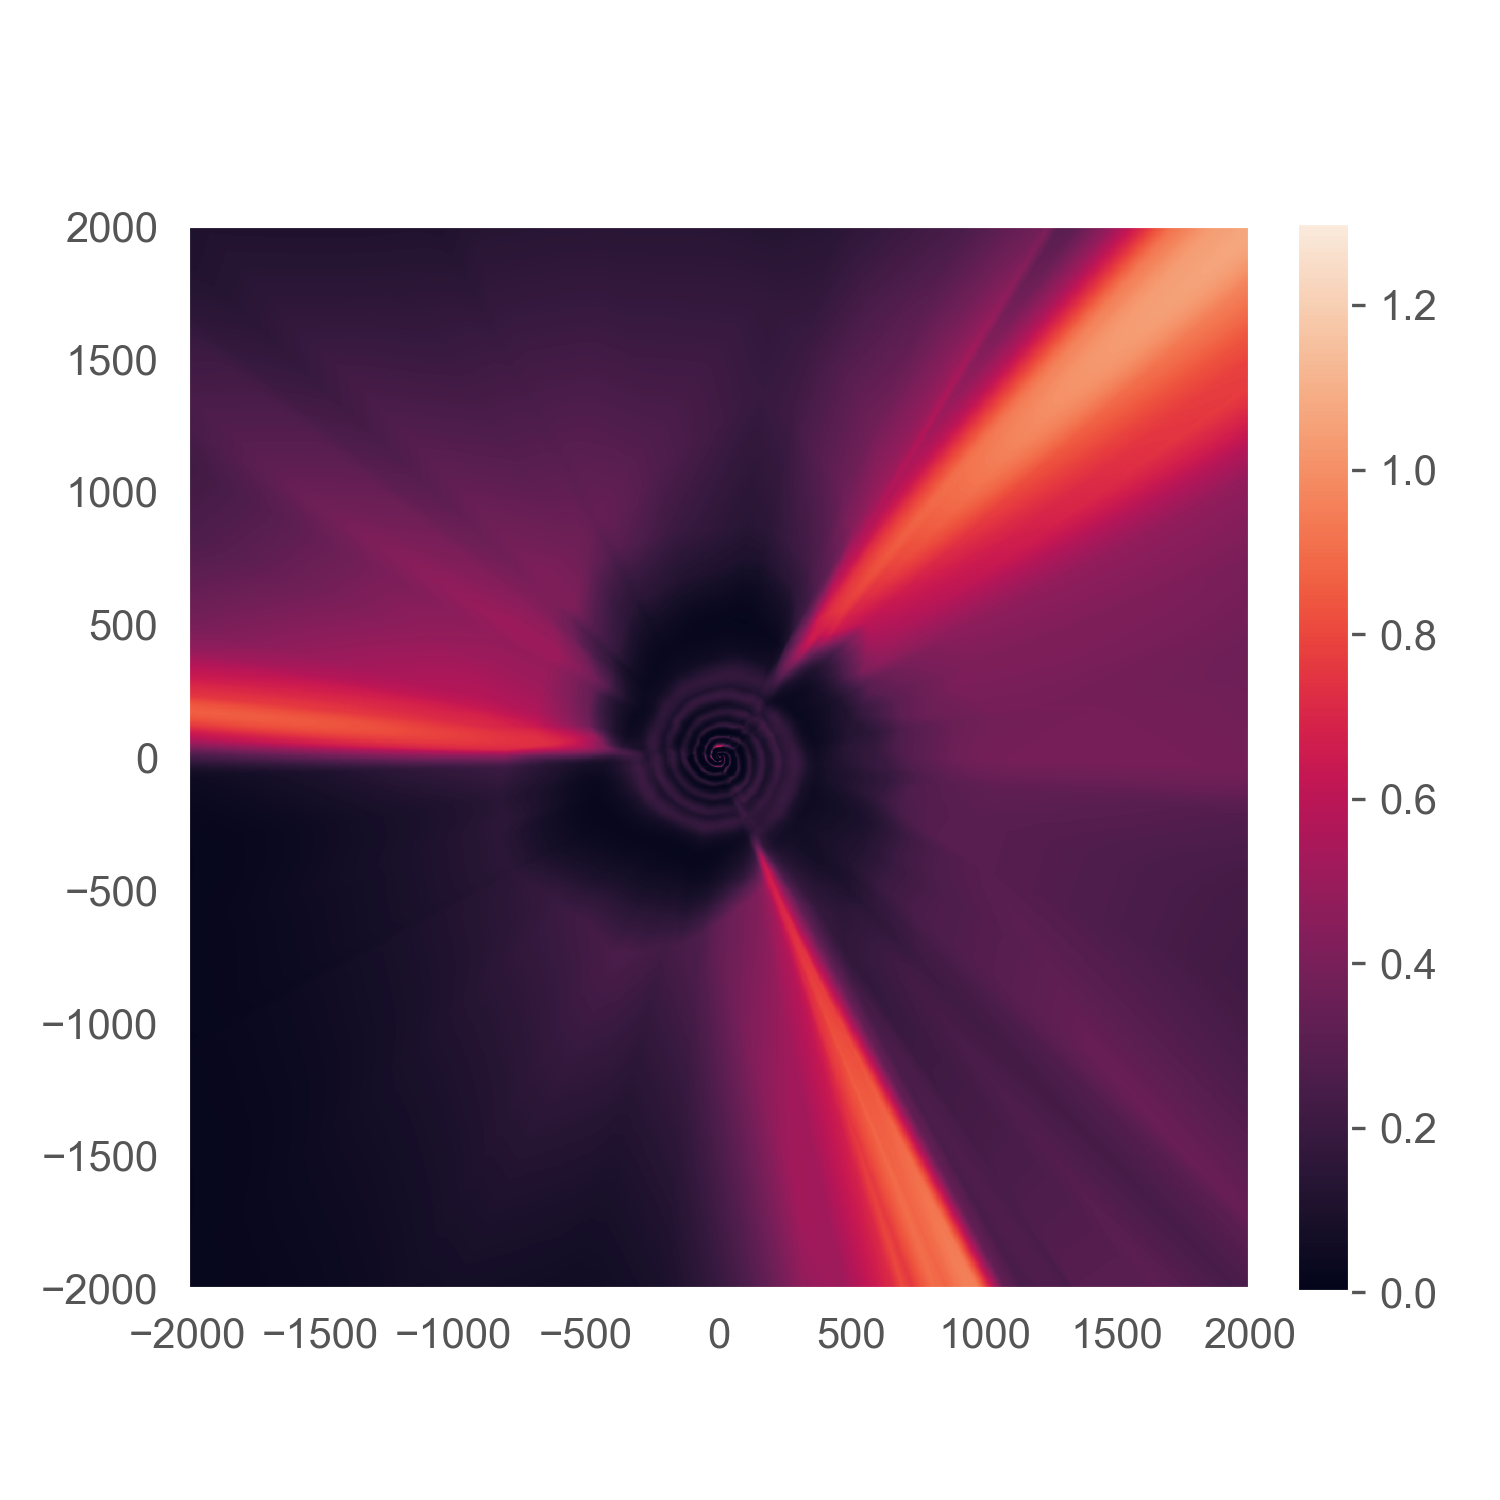
\includegraphics[trim=42 45 15 55, clip, width=\linewidth]{../openreview/plots/3l.png}
  \caption{EnD$^2_{\texttt{+AUX,ANN}}$ Know. Unct.}
  \label{fig:3i}
\end{subfigure}%

\begin{subfigure}{0.22\textwidth}
  \centering
  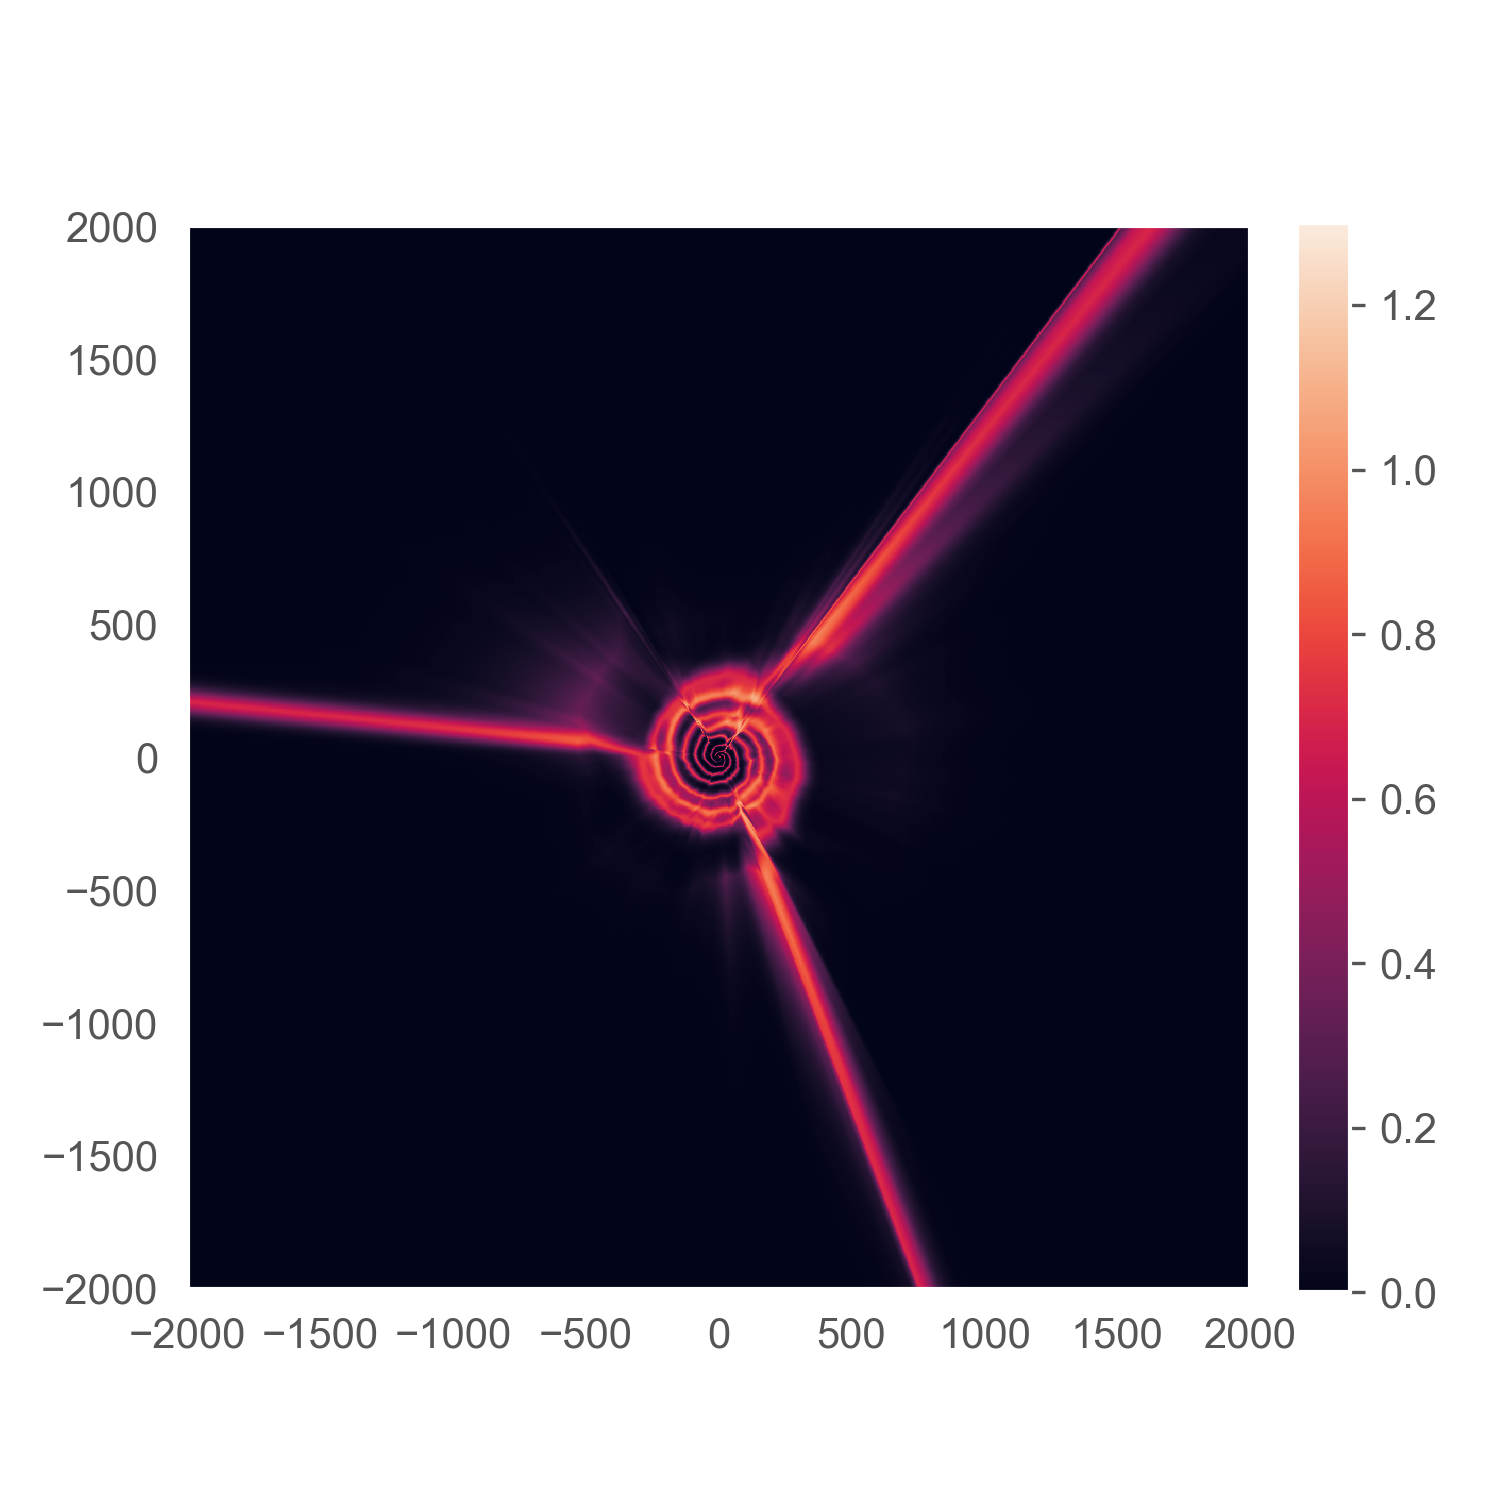
\includegraphics[trim=42 45 15 55, clip, width=\linewidth]{../openreview/plots/3m.png}
  \caption{EnD$^2_{\texttt{+AUX,T=2.5}}$ Tot. Unct.}
  \label{fig:3m}
\end{subfigure}%
\begin{subfigure}{0.22\textwidth}
  \centering
  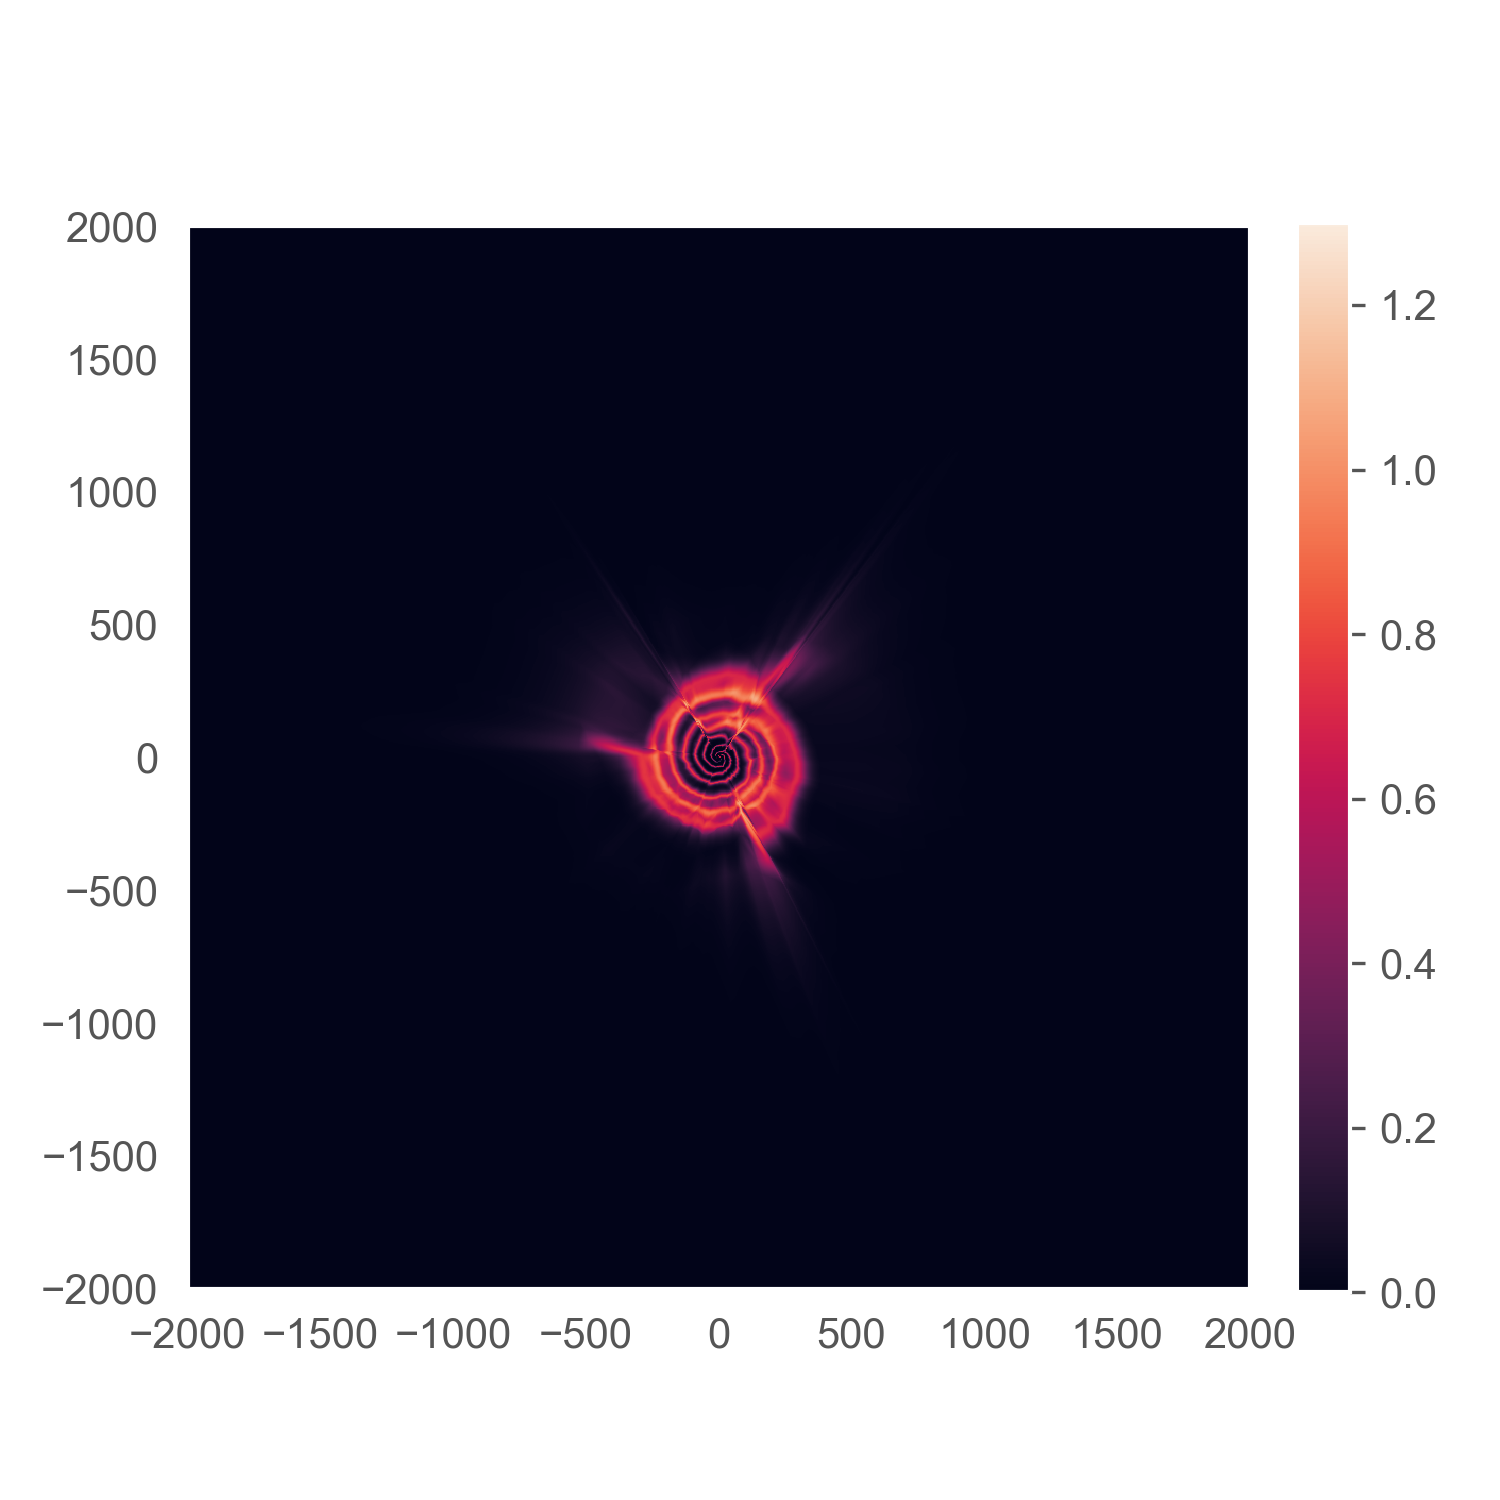
\includegraphics[trim=42 45 15 55, clip, width=\linewidth]{../openreview/plots/3n.png}
  \caption{EnD$^2_{\texttt{+AUX,T=2.5}}$ Data Unct.}
  \label{fig:3n}
\end{subfigure}%
\begin{subfigure}{0.22\textwidth}
  \centering
  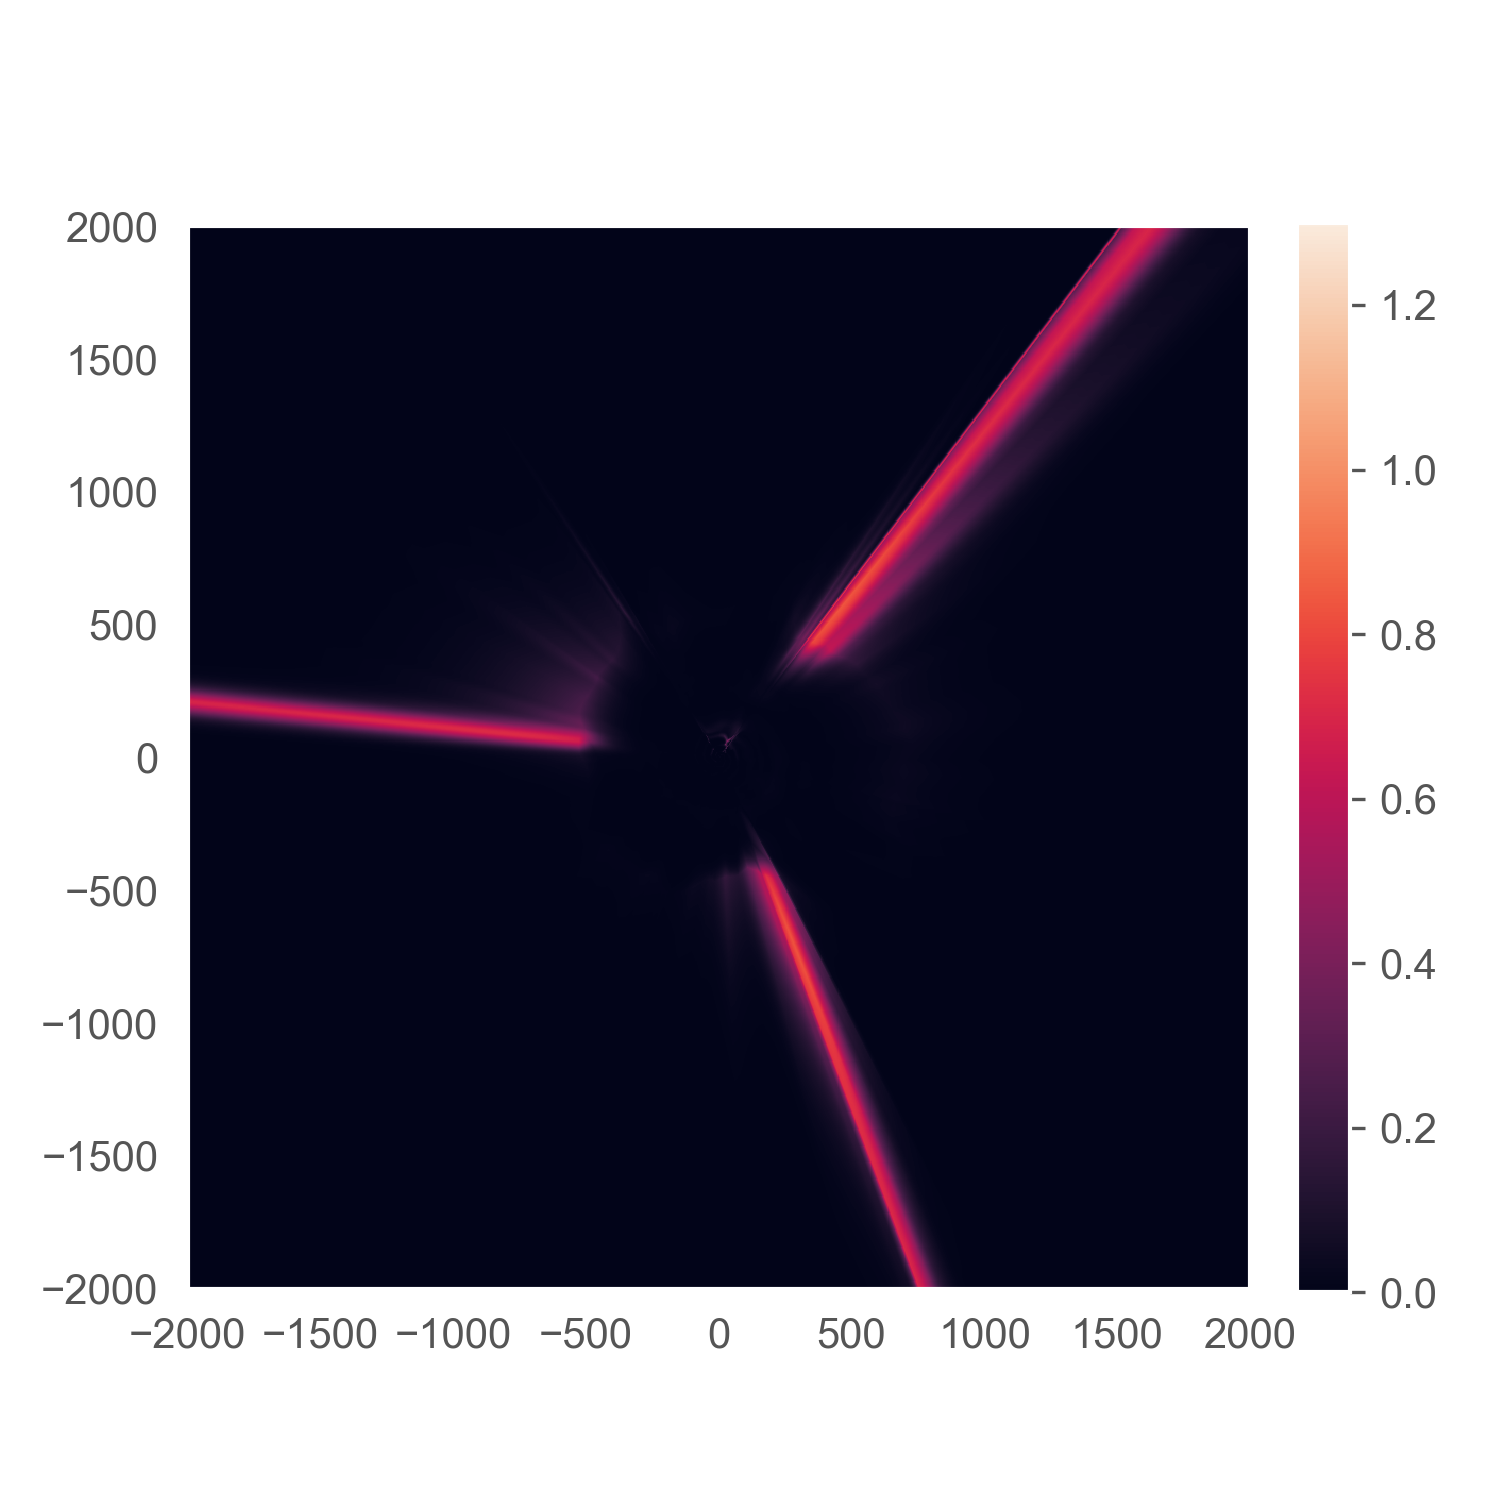
\includegraphics[trim=42 45 15 55, clip, width=\linewidth]{../openreview/plots/3o.png}
  \caption{EnD$^2_{\texttt{+AUX,T=2.5}}$ Know. Unct.}
  \label{fig:3o}
\end{subfigure}%

\begin{subfigure}{0.22\textwidth}
  \centering
  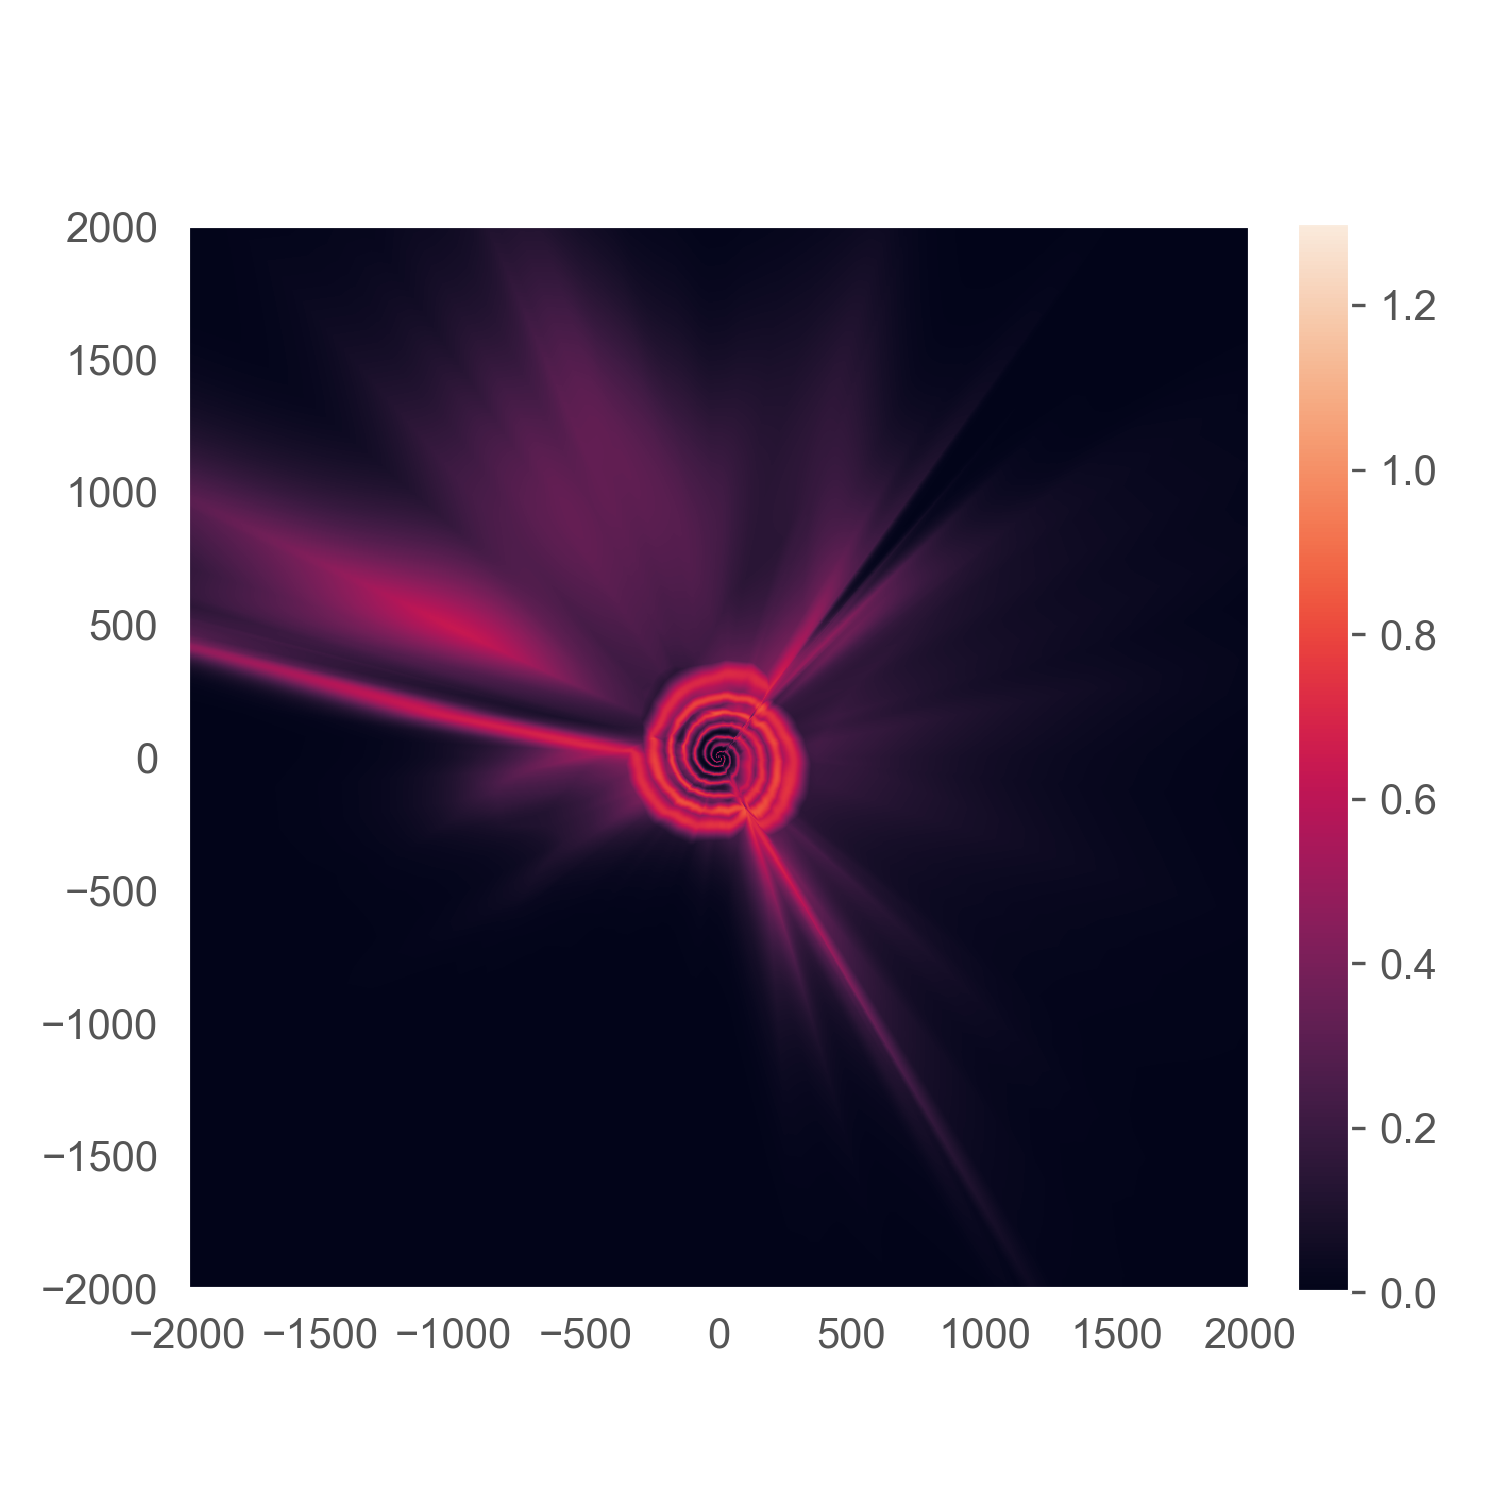
\includegraphics[trim=42 45 15 55, clip, width=\linewidth]{../openreview/plots/3q.png}
  \caption{EnD$^2_{\texttt{+AUX20}}$ Tot. Unct.}
  \label{fig:3p}
\end{subfigure}%
\begin{subfigure}{0.22\textwidth}
  \centering
  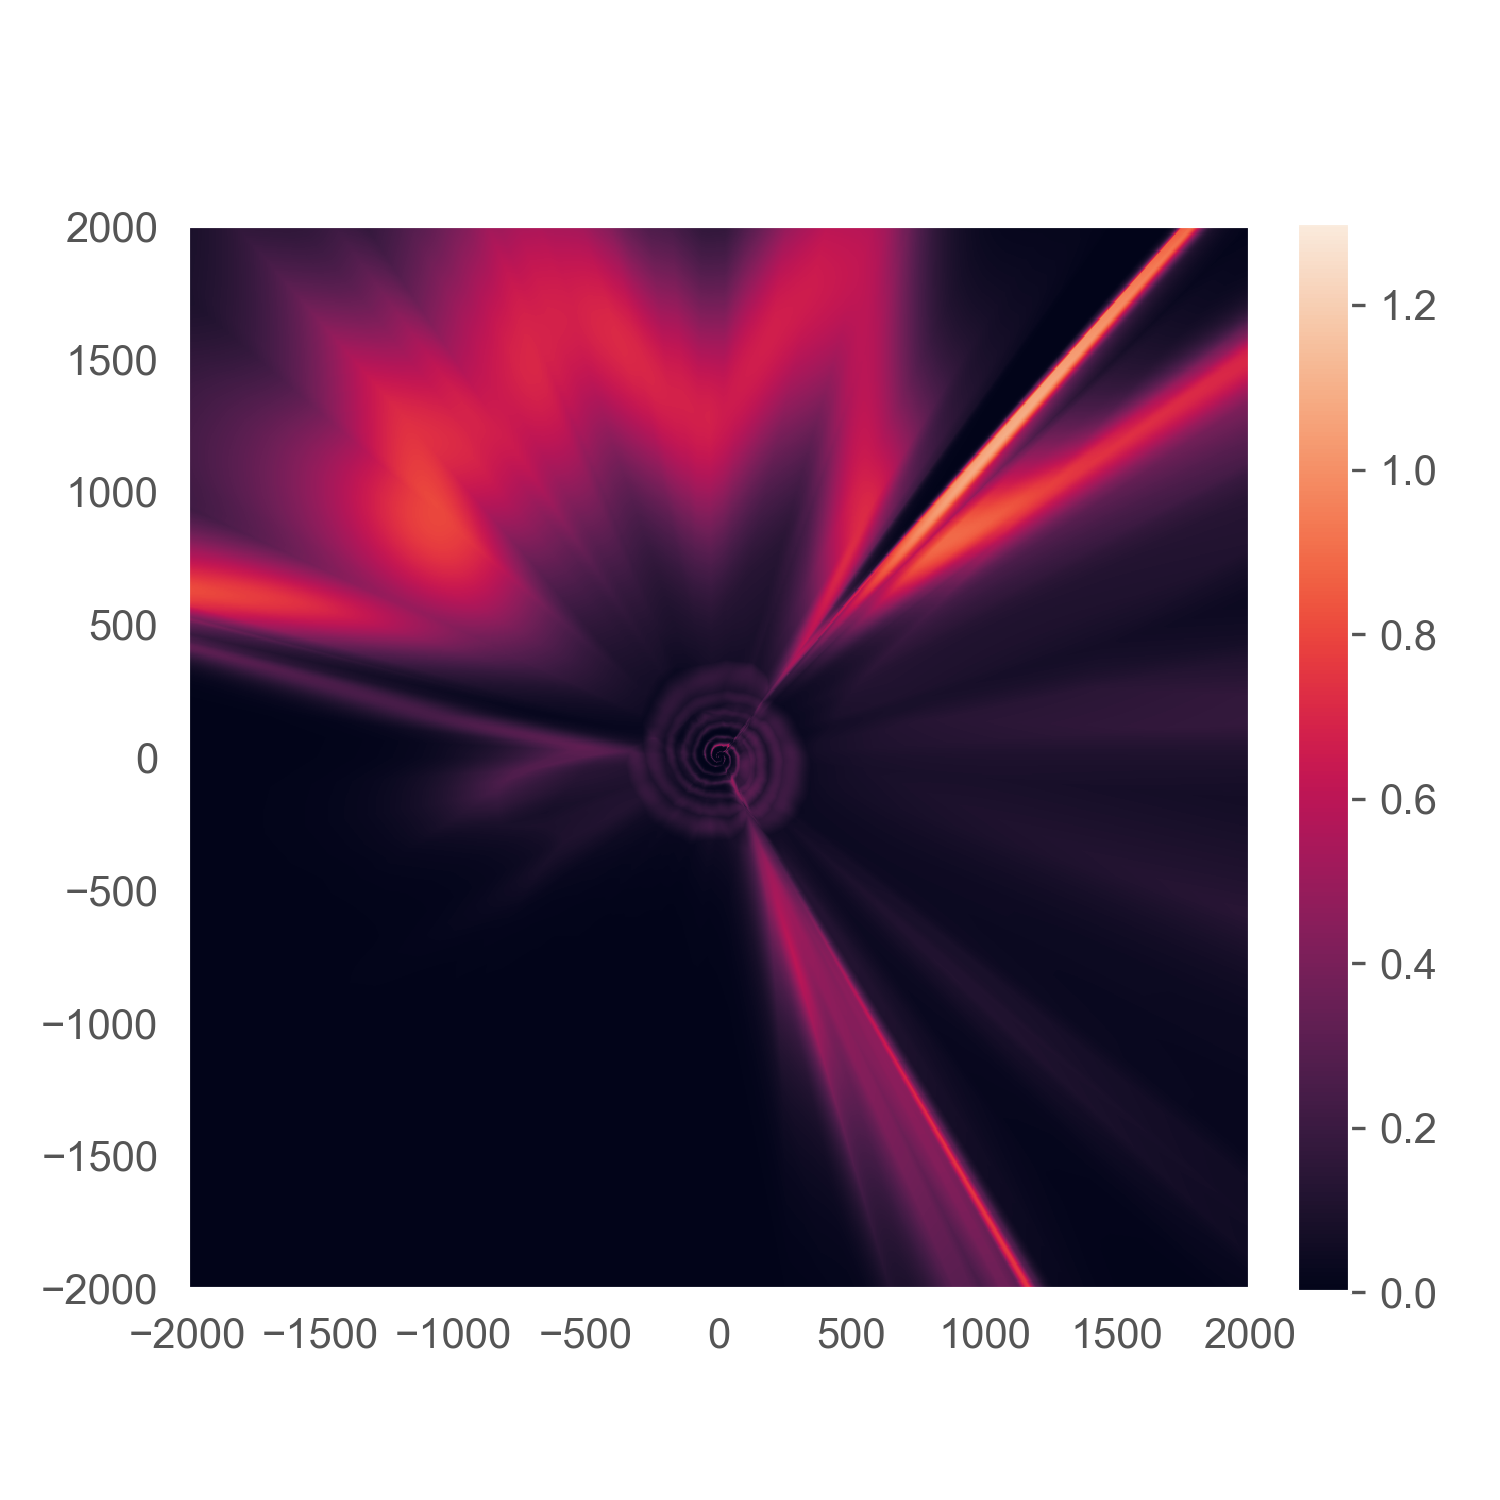
\includegraphics[trim=42 45 15 55, clip, width=\linewidth]{../openreview/plots/3r.png}
  \caption{EnD$^2_{\texttt{+AUX20}}$ Data Unct.}
  \label{fig:3q}
\end{subfigure}%
\begin{subfigure}{0.22\textwidth}
  \centering
  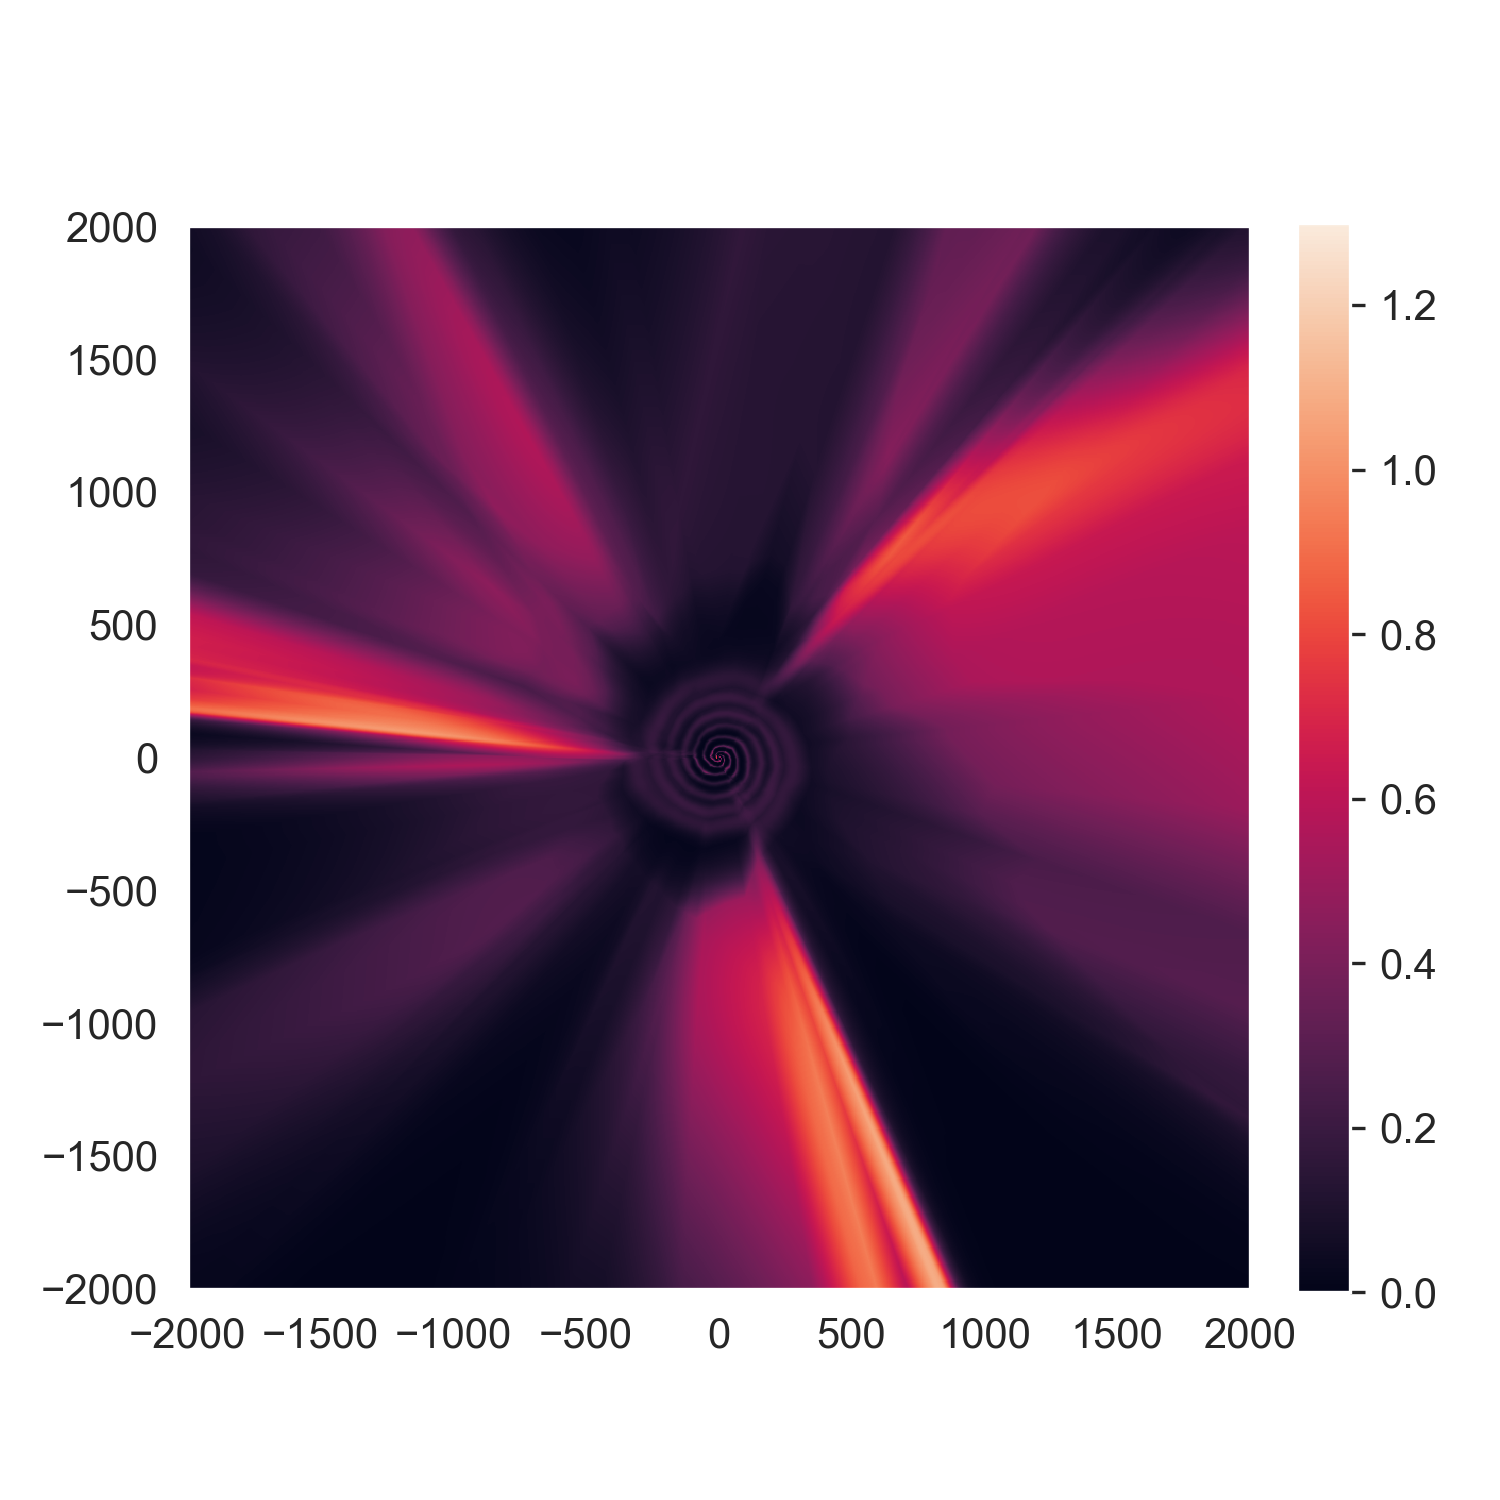
\includegraphics[trim=42 45 15 55, clip, width=\linewidth]{../openreview/plots/3s.png}
  \caption{EnD$^2_{\texttt{+AUX20}}$ Know. Unct.}
  \label{fig:3r}
\end{subfigure}%

\caption{Recreation of Figure 3 in \cite{malinin2019ensemble}, showing uncertainties over entire data manifold.}
\label{fig:fig3}
\end{figure}





\section{Computational requirements for reproduction}

In this section, we report the computational resources used for this reproduction. The running time of the major experiments on CIFAR-10 is expressed in time on an RTX 2070. For easier comparison, we also report the equivalent cost when running on a V100 GPU on Google Cloud for \$2.48 per hour, given a relative performance of 2.89 versus an RTX 2070\footnote{Benchmark taken from \url{https://timdettmers.com/2020/09/07/which-gpu-for-deep-learning/}}. Note that these figures represent the time to reproduce only the final experiments. We estimate that the total GPU time used for this reproduction, including experimentation and bug-hunting, to be 3 to 5 times as long. The full data can be seen in Table \ref{tab:comp}. 


\begin{table}[]
    \centering
     \caption{Computation requirements for major experiments, and which claims they test. GPU time refers to time on an NVIDIA GeForce RTX 2070. Equivalent cost represents the cost if run on a V100 on Google cloud, for \$2.48 per hour. }
    \begin{tabular}{l || r | r | r| r}
         \textbf{Experiment} & \textbf{Models} & \textbf{GPU min/model}  & \textbf{GPU days} & \textbf{Eqv. cost (USD)}  \\
         \hline
         \hline
         Ensemble, training & $400$ & $16$ & $4.44$ & $91.53$\\
         Ensemble, labeling & $400$& $0.45$ & $0.13$ & $2.57$\\
         Ensemble, inference & $400$& $0.23$ & $0.06$ & $1.32$ \\
         \hline 
         Evaluation, \hyperlink{claim1}{claim 1 and 2} & 15 & 51 & 0.53 & 10.94 \\
         \hline
         Size ablation, training, \hyperlink{claim3}{claim 3} & $112$ & $51$ & $3.97$ & $81.69$ \\
         Temperature ablation, training, \hyperlink{claim4}{claim 4} & $27$ & $51$ & $0.96$& $19.69$\\
         \hline
         3-class ensemble, training, \hyperlink{claim 5}{claim 5} &100 &5.25 &0.36 &7.51 \\
         \hline
         \hline
         \textbf{Total} & & & $11.413$ & $235.06$
    \end{tabular}
   
    \label{tab:comp}
\end{table}


\section{Histograms}
To compare ensembles, \EnDD \ and \EnDDaux \ on the CIFAR-10 and 3-class CIFAR-10 datasets, we provide histograms of data and knowledge uncertainty for in- and out-of-domain-distribution, in Figure \ref{fig:uncertainty_hist} and \ref{fig:3-class_uncertainty_hist}. 


\section{Relative performance of \EnDD \ compared to ensemble and original article}

In Tables 3 and 4 of the main report we report several measures for the 7 different models tested. For better comparability, we here also provide the values normalized to the ensembles' performance, both for our experiments, and for the original paper, in Table \ref{tab:classification-measures-norm} and \ref{tab:ood-measures-norm}. 




\begin{table}
\centering
\caption{OOD ROC-AUC$\uparrow$ on CIFAR-10 (in) and LSUN (out), normalized to ensemble results. Error bounds signify two standard deviations, taken over three models.}
\addtolength{\leftskip} {-3cm}
\addtolength{\rightskip}{-3cm}
\begin{tabular}{r||r|r|r|r|r|r|r} 
\hline
Unc. & IND & ENSM & EnD & $\text{EnD}^2$ & EnD$_\texttt{+AUX}$ & \EnDDaux & PN $_\texttt{+AUX}$ \\ [0.5ex] 
\hline
\hline
Tot. our&
$0.96 \scriptstyle \pm 0.00$ &
$1.00 \scriptstyle \pm NA$ &
$1.00 \scriptstyle \pm 0.01$ &
$0.98 \scriptstyle \pm 0.00$ &
$1.01 \scriptstyle \pm 0.00$ &
$1.00 \scriptstyle \pm 0.00$ &
$\mathbf{1.02} \scriptstyle \pm 0.01$ \\ 

Tot. paper&
$0.97 \scriptstyle \pm 0.01$ &
$1.00 \scriptstyle \pm NA$ &
$0.94 \scriptstyle \pm 0.01$ &
$0.97 \scriptstyle \pm 0.01$ &
$0.94 \scriptstyle \pm 0.01$ &
$1.00 \scriptstyle \pm 0.01$ &
$\mathbf{1.01} \scriptstyle \pm 0.01$ \\ 

\hline

Know., our&
- &
$1.00 \scriptstyle \pm NA$ &
- &
$0.95 \scriptstyle \pm 0.01$ &
- &
$0.99 \scriptstyle \pm 0.01$ &
$\mathbf{1.02} \scriptstyle \pm 0.00$ \\

Know., paper&
- &
$1.00 \scriptstyle \pm NA$ &
- &
$0.98 \scriptstyle \pm 0.01$ &
- &
$0.99 \scriptstyle \pm 0.01$ &
$\mathbf{1.01} \scriptstyle \pm 0.01$ \\ 
\hline
\end{tabular}
\\ [1ex] 
\label{tab:ood-measures-norm}
\end{table}

\begin{figure}[h!]
    \centering
    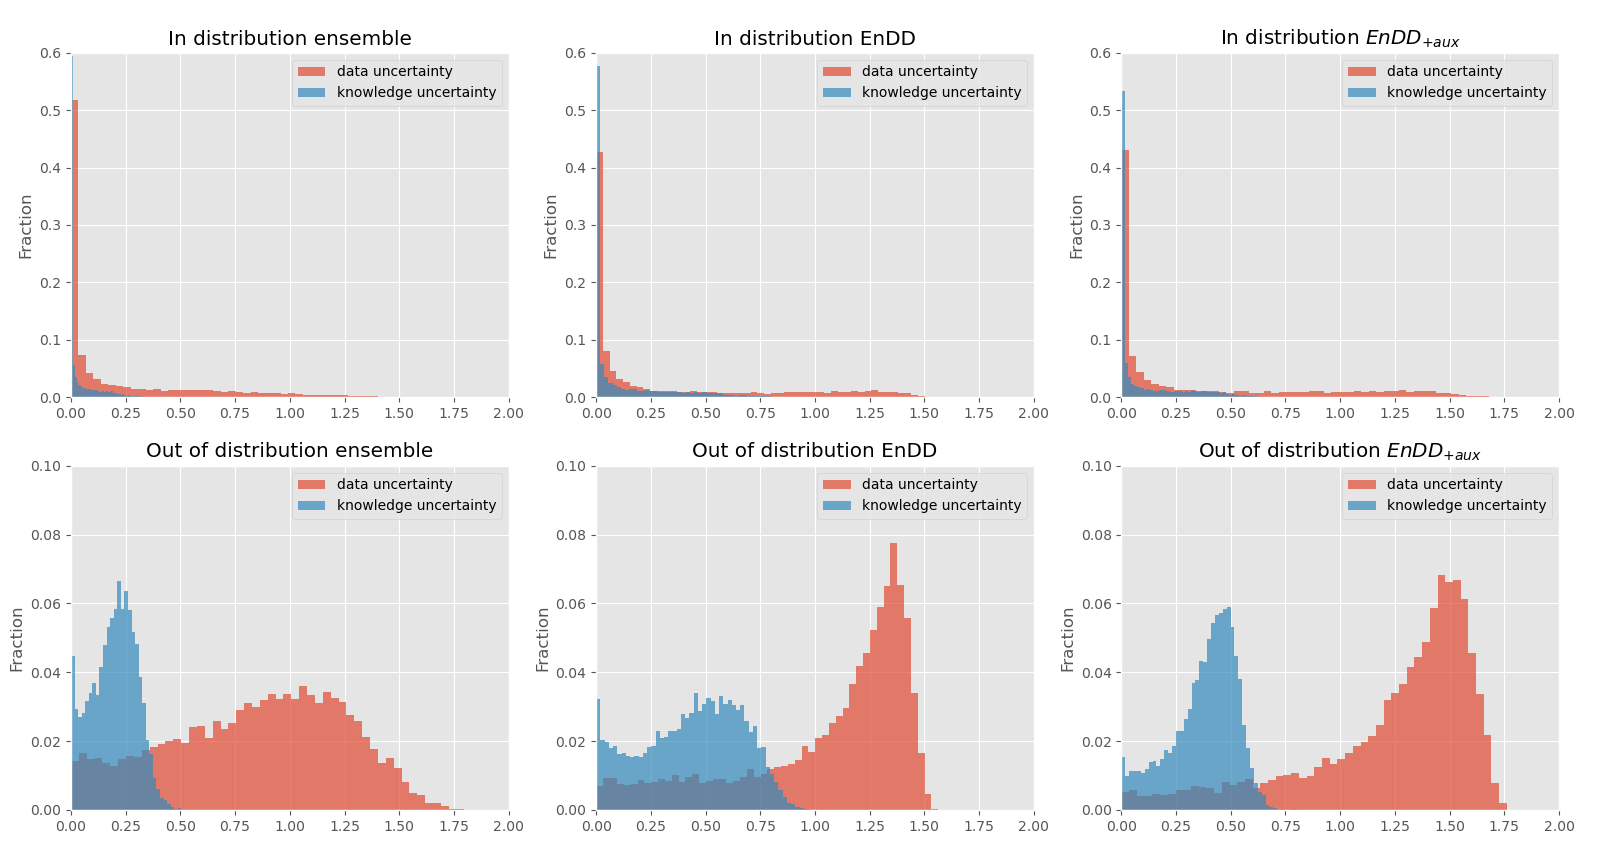
\includegraphics[width = \linewidth]{../openreview/plots/uncertainty_hist_all.PNG}
    \caption{Data/knowledge uncertainty-distributions for ensemble, \EnDD \ and \EnDDaux.}
    \label{fig:uncertainty_hist}
\end{figure}

\begin{figure}[h!]
    \centering
    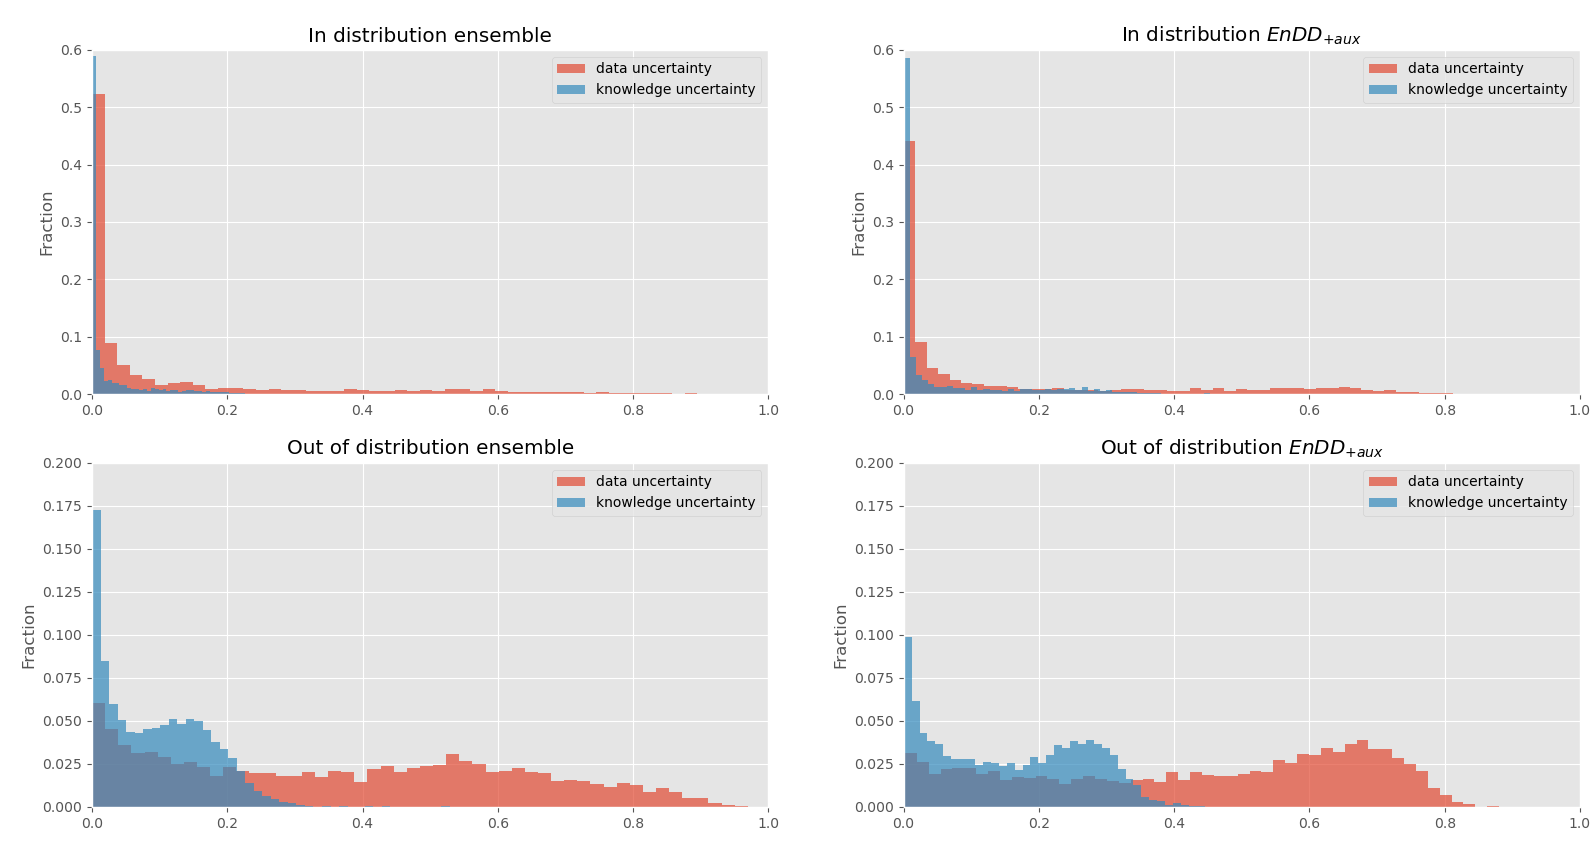
\includegraphics[width = \linewidth]{../openreview/plots/uncertainty_hist_3class.PNG}
    \caption{Data/knowledge uncertainty-distributions for ensemble and \EnDDaux \ on the 3-class CIFAR10 dataset}
    \label{fig:3-class_uncertainty_hist}
\end{figure}



\begin{table}
\centering
\caption{Classification metrics on CIFAR-10, normalized to ensemble results. Error bounds signify two standard deviations, taken over three models.}
\addtolength{\leftskip} {-3cm}
\addtolength{\rightskip}{-3cm}
\begin{tabular}{r||r|r|r|r|r|r|r} 
\hline
Crit. & IND & ENSM & EnD & $\text{EnD}^2$ & EnD$_\texttt{+AUX}$ & \EnDDaux & PN$_\texttt{+AUX}$ \\ [0.5ex] 
\hline
\hline
ERR$\downarrow$, our & 
$1.12 \scriptstyle \pm 0.08$ &
$1.00 \scriptstyle \pm NA$ &
$\mathbf{0.99} \scriptstyle \pm 0.06$ &
$1.13 \scriptstyle \pm 0.02$ &
$1.13 \scriptstyle \pm 0.02$ &
$1.16 \scriptstyle \pm 0.01$ &
$1.14 \scriptstyle \pm 0.04$ \\ 

ERR$\downarrow$, paper & 
$1.29 \scriptstyle \pm 0.06$ &
$\mathbf{1.00} \scriptstyle \pm NA$ &
$1.08 \scriptstyle \pm 0.05$ &
$1.18 \scriptstyle \pm 0.03$ &
$1.08 \scriptstyle \pm 0.03$ &
$1.11 \scriptstyle \pm 0.06$ &
$1.21 \scriptstyle \pm 0.10$ \\ 

\hline

PRR$\uparrow$, our & 
$0.87 \scriptstyle \pm 0.02$ &
$\mathbf{1.00} \scriptstyle \pm NA$ &
$0.98 \scriptstyle \pm 0.00$ &
$0.96 \scriptstyle \pm 0.01$ &
$0.98 \scriptstyle \pm 0.02$ &
$0.96 \scriptstyle \pm 0.01$ &
$0.70 \scriptstyle \pm 0.12$ \\ 

PRR$\uparrow$, paper & 
$0.97 \scriptstyle \pm 0.01$ &
$\mathbf{1.00} \scriptstyle \pm NA$ &
$0.98 \scriptstyle \pm 0.01$ &
$0.98 \scriptstyle \pm 0.01$ &
$0.98 \scriptstyle \pm 0.00$ &
$0.99 \scriptstyle \pm 0.00$ &
$0.94 \scriptstyle \pm 0.02$ \\ 

\hline

ECE$\downarrow$, our &
$41.37 \scriptstyle \pm 0.35$ &
$1.00 \scriptstyle \pm NA$ &
$\mathbf{0.94} \scriptstyle \pm 0.05$ &
$1.45 \scriptstyle \pm 0.13$ &
$1.08 \scriptstyle \pm 0.19$ &
$1.85 \scriptstyle \pm 0.29$ &
$5.69 \scriptstyle \pm 0.37$ \\

ECE$\downarrow$, paper &
$1.69 \scriptstyle \pm 0.31$ &
$1.00 \scriptstyle \pm NA$ &
$2.00 \scriptstyle \pm 0.15$ &
$\mathbf{0.77} \scriptstyle \pm 0.15$ &
$2.00 \scriptstyle \pm 0.46$ &
$1.69 \scriptstyle \pm 0.31$ &
$9.23 \scriptstyle \pm 0.54$ \\

\hline

NLL$\downarrow$, our &
$6.38 \scriptstyle \pm 0.04$ &
$\mathbf{1.00}\scriptstyle \pm NA$ &
$1.06 \scriptstyle \pm 0.04$ &
$1.35 \scriptstyle \pm 0.02$ &
$1.19 \scriptstyle \pm 0.01$ &
$1.38 \scriptstyle \pm 0.01$ &
$1.86 \scriptstyle \pm 0.04$ \\ 

NLL$\downarrow$, paper &
$1.32 \scriptstyle \pm 0.05$ &
$\mathbf{1.00}\scriptstyle \pm NA$ &
$1.16 \scriptstyle \pm 0.05$ &
$1.32 \scriptstyle \pm 0.05$ &
$1.16 \scriptstyle \pm 0.05$ &
$1.26 \scriptstyle \pm 0.00$ &
$2.00 \scriptstyle \pm 0.05$ \\ 
\hline
\end{tabular}
\\ [1ex] 

\label{tab:classification-measures-norm}
\end{table}




